\documentclass[10pt,twoside]{book}
\usepackage[a4paper]{anysize}
\usepackage[portuguese, english]{babel}
\usepackage[ansinew,utf8]{inputenc}
\usepackage{amsmath,amssymb,amsthm,amsfonts,mathrsfs,cite,color,enumerate,epsfig,yfonts,fancyhdr,graphicx,makeidx,textcomp}
\usepackage[all]{xy}
% \usepackage{draftwatermark}

\usepackage{hyperref}
\hypersetup{
%     bookmarks=true,         % show bookmarks bar?
%     bookmarksnumbered=true,
    unicode=true,          % non-Latin characters in Acrobat’s bookmarks
%     pdftoolbar=true,        % show Acrobat’s toolbar?
%     pdfmenubar=true,        % show Acrobat’s menu?
%    pdffitwindow=false,     % window fit to page when opened
    pdfstartview={FitH},    % fits the width of the page to the window
    pdftitle={On the existence of categorical connections},    % title
    pdfauthor={Nelson Batalha},     % author
    pdfsubject={Differential Geometry},   % subject of the document
%    pdfcreator={Creator},   % creator of the document
%    pdfproducer={Producer}, % producer of the document
%    pdfkeywords={keywords}, % list of keywords
    pdfnewwindow=false,      % links in new window
    colorlinks=false,       % false: boxed links; true: colored links
    linkcolor=black,          % color of internal links
    citecolor=black,        % color of links to bibliography
    filecolor=black,      % color of file links
    urlcolor=black           % color of external links
}



\newtheorem{theorem}{Theorem}[section]
\newtheorem{definition}[theorem]{Definition}
\newtheorem{example}[theorem]{Example}
\newtheorem{remark}[theorem]{Remark}
\newtheorem{prop}[theorem]{Proposition}
\newtheorem{lemma}[theorem]{Lemma}
\newtheorem{corollary}[theorem]{Corollary}%[chapter]
\newenvironment{proof2}{\noindent {\sc Proof:}}{$\,\hfill \Box$\smallskip}

\newtheorem{step}{Step}

\def\of #1{\!\left({#1}\right)}
\def\hol {{\rm hol}}

\newcommand{\fpartial}[2]{\frac{\partial #1}{\partial #2}}
\newcommand{\towrite}{\begin{center}{\Large $\clubsuit$ Section not yet written
$\clubsuit$ } \end{center}}
\newcommand{\tofinish}{\begin{center} {\Large $\spadesuit$ Section not yet
finished $\spadesuit$}\end{center}}
\newcommand{\notsure}[1]{\emph{#1}\footnote{$\clubsuit$CONFIRM$\clubsuit$}}
\newcommand{\improve}[1]{\begin{center}
                         \begin{tabular}{|p{8cm}|}
\hline
\textbf{TO DO}: \textsc{#1}\\
\hline
\end{tabular}
                         \end{center}}
%\newcommand{\future}[1]{{\color{red} #1}}
\newcommand{\future}[1]{}
\newcommand{\question}[1]{\begin{center}
                         \begin{tabular}{|p{8cm}|}
\hline
\textbf{\textsc{Q}}: {\color{red} \textsc{#1}}\\
\hline
\end{tabular}
                         \end{center}}
\newcommand{\squestion}[1]{\footnote{$\clubsuit\spadesuit$#1$\clubsuit\spadesuit$}}
\newcommand{\define}[1]{\index{#1}\emph{#1}}
\newcommand{\mention}[1]{\index{#1} \emph{#1}}




%% \SetWatermarkFontSize{10cm}
%% \SetWatermarkScale{4}
%% \SetWatermarkLightness{0.95}



\makeindex

\begin{document}
\shorthandoff{"} % Hack to run babel portuguese and xypic

\thispagestyle{empty}
\selectlanguage{portuguese}
\begin{figure}[t]
\begin{picture}(90,23)(0,0)

  \put(-30,5){
\includegraphics[scale=0.584]{figures/istsymbol.pdf}}

\end{picture}
 
\end{figure}

\vspace*{1cm}


\begin{center}

\mbox{{\LARGE \textbf{On the existence of categorical connections}  }}
\vspace{0.2cm} 

%\mbox{{\LARGE \textbf{Minimum Energy Estimator}  }}
\vspace{0.3cm} 

\vspace{3cm}

\mbox{\bf {\Large Nelson Batalha}}\\


\vspace{4cm}

\mbox{\LARGE Dissertação para obtenção do Grau de Mestre em}\\
\vspace{0.3cm}
\mbox{\bf {\LARGE Matemática e Aplicações}}\\


\vspace{3cm}

\mbox{\textbf{\Large Júri}}
\end{center}


\vspace{-0.3cm}


\begin{table}[h]
\begin{tabular}{l l l}
&\large Presidente: &\large Prof. Dr. Rui Loja Fernandes \\
&\large Orientador: &\large Prof. Dr. Gustavo Rui de Oliveira Granja \\
&\large Vogais: &\large Prof. Dr. Roger Francis Picken \\
&\large \phantom{Vogais:} &\large Prof. Dr. João Nuno Gonçalves Faria Martins  \\
\end{tabular}
\end{table}


\vspace*{-0.3cm}

\begin{center}
\textbf{{\large Julho de 2010}}
\end{center}




\thispagestyle{empty}


\newpage
\thispagestyle{empty}
\mbox{$\,$}
\newpage
\thispagestyle{empty}
$\,$
\vskip7.3cm
\begin{flushright}
\emph{The universe is full of magical things, patiently waiting for our wits to grow sharper}\\
Eden Philpotts
\end{flushright}

\frontmatter
\selectlanguage{english}
\parbox[t][2cm][c]{\textwidth}{~\vfill}
\section*{Acknowledgements}

\addcontentsline{toc}{section}{Acknowledgements}

I am in great debt to the talented teachers I have encountered in this faculty and before who inspired me to get this far.

In particular, this thesis would not have been written without the fantastic support from my advisor Professor Gustavo Granja, whose patience and contributions far exceed anything I could have asked.

Also I would like to thank my colleagues for the helpful discussions and insights, and my family and friends who made it possible.

Special thanks to Professor John Baez for making available online so much (and diverse) material contagiously passionate, and to Professor Roger Picken and colleagues whose articles were the reason this study started.
\selectlanguage{english}
\parbox[t][2cm][c]{\textwidth}{~\vfill}
\section*{Abstract}
\addcontentsline{toc}{section}{Abstract}

We review the construction of 2-bundles with 2-connections by Baez as a categorification of locally trivial principal bundles with connections and focus our study on the particular case of categorical connections. Namely we study conditions for their existence.

\vfill
\textbf{\Large Keywords:} 2-bundle, 2-categories, categorical connection, categorification, internalization, higher gauge theory, holonomy.

\selectlanguage{portuguese}
\parbox[t][2cm][c]{\textwidth}{~\vfill}
\section*{Resumo}

\addcontentsline{toc}{section}{Resumo}

Revemos a construção de 2-fibrados com 2-conexões de Baez como uma categorificação de fibrados principais localmente triviais com conexões e focamos o nosso estudo no caso particular das conexões categóricas. Nomeadamente estudamos condições para a sua existência.
\vfill

\textbf{\Large Palavras-chave:} 2-categorias, 2-fibrado, categorifica\c{c}\~ao, conexão categórica, internaliza\c{c}\~ao, holonomia, teoria de gauge superior.

\selectlanguage{english}
\newpage
%\include{notation/notation}


%\listoffigures
%\listoftables

\newpage

\selectlanguage{english}
 \setcounter{tocdepth}{2}
\tableofcontents
\addcontentsline{toc}{chapter}{Index}

\newpage
\mainmatter

%\include{sites/sites}
\chapter*{Introduction}

Gauge theory is a mathematical theory that describes the evolution of the state of point particles. Recently, in physics, the need to describe the evolution of more complicated objects such as strings has led to the development of the new field of higher gauge theory.

In this thesis we will give an overview of this field with particular focus on the special case of categorical connections and holonomies which have recently been introduced by Martins and Picken.

In \textbf{Section 1}, we review the basic concepts necessary for the remaining chapters. We begin by introducing 2-categories, which are basically categories together with ``morphisms of morphisms''. Notice that in regular categories one can talk of \emph{isomorphisms} between objects using arrows, however one can only discuss \emph{equalities} of morphisms as elements in a set. By introducing morphisms of morphisms, a notion of isomorphism of arrows is naturally introduced, leaving only the equality relation on $2$-morphisms.

Using this notion of isomorphism of arrows, we could also extend, say, the associativity relation of the composition rule to an equality \emph{up to isomorphism}. This would lead us to \define{weak  2-categories} (or bicategories) as in \cite{maclane} and \cite{ncatsbaez}. As shown in this last paper, these provide a more natural framework than strict categories, but at the time of writing there isn't either a well established definition of what a weak $n$-category (for $n\geq 3$), nor for that matter, what a 2-bundle with a such a weak group is. Here, we will consider only \emph{strict} 2-categories.

$n$-Categories are closely related to the theory of Categorification (\cite{categorification}). Quoting  Baez and Dolan:
\begin{quote}
 Categorification is the process of finding category-theoretic analogs
of set-theoretic concepts by replacing sets with categories, functions with functors, and equations between functions by natural isomorphisms between functors, which in turn should satisfy certain equations of their own, called ``coherence laws''. Iterating this process requires a theory of ``n-categories'', algebraic structures having objects, morphisms between objects, 2-morphisms between morphisms and so on up to n-morphisms.
\end{quote}

Our main goal is to study categorifications of bundles with connections, which we review in \textbf{Section 2} without proofs.

In \textbf{Section 3} we begin by introducing the construction of $2$-bundles with connection by Baez and Schreiber (\cite{baez-2004}), as in their introductory paper \cite{baezhigher}. Following the instructions above, a categorification of a bundle should be a functor $p:E\rightarrow B$ between some categories $E$ and $B$. This leads us to a structure ``2-group'' $G$. These should still have some differentiable structure, with an added group like structure in $G$. Baez's approach uses the concept of internal category by Ehresmann (\cite{ehresmann}), wherein given a category $K$, we write the axioms for the algebraic structure present in a category in terms of commutative diagrams and interpret these in $K$.

%%roughly a category whose objects and morphisms are objects in another category. 
% 
% These internal categories together with ``internal'' functors and natural transformations form a 2-category. Also, since a group can be thought as category $\mathcal{G}$ with one object and invertible morphisms, by categorifying it we get a 2-category. 

Coincidentally this abstract construction leads to a natural way of describing certain concepts which are important in string theory, much in the way that bundles and connections are used to describe classical physics. Whereas holonomy assigned to each path of a particle a group element $g$, or in categorical terms a morphism 
\[
 \xymatrix{ \bullet \ar@/^1pc/[r]^g & \bullet}
\]
our categorified holonomy (or 2-connection) will be a functor assigning to both paths and ``surfaces'' (say the area swept by a 1-dimensional string) a morphism and a 2-morphism in our 2-group

\[
 \xymatrix{ \bullet \ar@/^1pc/[rr]^{g}_{}="0"
           \ar@/_1pc/[rr]_{g'}="1"
           \ar@{=>}"0";"1"^{h} && \bullet}
\]
The foremost examples for physics have been very recently described in \cite{baezinvitation}. 
%Bundle-gerbes are another categorification of bundles carried by Murray (\cite{murray1,murray2}) not introduced here, built specifically to obtain objects \notsure{more directly usable in physics}.

We briefly mention the particular case of gerbs, which were studied in \cite{chatterjee} as a categorification of the cocycle condition that defines isomorphism classes of line bundles. This in turn is a particular case of the original construction of Giraud \cite{giraud}, and later Brylinski \cite{brylinski}.

Then we move on to a particular type of 2-connections, the categorical connections. Here lies the original part of this work, where we answer a question left open in \cite{picken_faria}. We study the existence of categorical connections in a given bundle and crossed module, by essentially describing categorical connections as sections in an associated vector bundle. 
This section can be read as an \emph{intermezzo} to the above article of Martins and Picken, who then proceed to construct categorical holonomies for each categorical connection. With this work, a criteria for the existence of categorical holonomies from categorical connections is immediate.
% 
% We take no credit
% 
% \improve{meter: we take no credit in sections (...) which we borrowed from ... for a short introduction.}
% \improve{finish this in the end}

\subsubsection*{Requisites} General Topology, Basic Category Theory and Differential Geometry.

\subsubsection*{Notation} We write $U_{i_1,\ldots,i_k}= U_{i_1}\cap\ldots \cap U_{i_k}$ with each $U_i$ open. By neighborhood we always mean an open neighborhood. When $G, H, \ldots$ are Lie groups, we denote the corresponding Lie algebras by $\mathfrak{g},\mathfrak{h}, \ldots$. For a category $C$, we denote $C_0$ its class of objects and $C_1$ its class of morphisms. By \define{$\textbf{Diff}$} we mean the category of smooth manifolds with smooth maps, which in turn we simply call spaces and maps. Often we write the composition of arrows from left to right, that is if $f:A\rightarrow B$ and $g:B\rightarrow C$ are composible morphisms, we denote the composition by $f\circ g$.

\subsubsection*{Assumptions}

The manifolds used here are assumed to be Hausdorff and second-countable.



\chapter{Prerequisites}
%\subsection{2-Categories}

A discussion of this definition can be found in \cite{maclane} (pgs. 273-275) and \cite{ncatsbaez}.

\future{hipotese de haver produtos, a terminal object e limites em $\mathbf{CAT}$ etc.}
\future{\improve{definicao confusa. A definicao mais recente e a partir de $\infty$-category, se houver tempo e nao complicar intuicao, entao reescrever. ou entao reescrever da forma mais longa uma introducao natural com diagramas (em baixo) como no maclane e depois resumir a definicao formal em baixo}}


\begin{definition}
A \define{2-category}, or a \define{strict 2-category}, consists of a category $C$, together with \begin{enumerate}
 \item categories $T(a,b)$ for all objects $a,b\in C_0$, where the objects of the category $T(a,b)$ are the morphisms in $C$ from $a$ to $b$,
\item a functor $F_{a,b,c}:T(a,b)\times T(b,c)\rightarrow T(a,c)$, for each triple of objects $a,b,c$ (the \define{horizontal composition}, denoted by $\circ$), that acts on objects as the usual composition of morphisms, is associative and satisfies the unity axioms (see below),
\item for each object $a$, a functor $U_a:1\rightarrow T(a,a)$, where $1$ is the terminal category (assigning to the single object of $1$ the identity morphism in $T(a,a)$).
\end{enumerate}
\end{definition}


Here we are adding to a category a collection of morphisms between morphisms that can be ``vertically'' composed. We refer to the arrows of $T(a,b)$ as the \define{$2$-morphisms} or \define{$2$-cells}, which inherit from $T(a,b)$ the \define{vertical composition} denoted by $\bullet$. For a 2-morphism $\alpha$ from $f:a\rightarrow b$ to $g:a\rightarrow b$, we write $\alpha: f\Rightarrow g$, or 

\[
 \xymatrix{a \ar@/^1pc/[rr]^{f}_{}="0"
           \ar@/_1pc/[rr]_{g}="1"
           \ar@{=>}"0";"1"^{\alpha}
&& b
}
\]

For each $f:a\rightarrow b$, \define{$id_f$}\footnote{Often we make the abuse of just writing $f$.} denotes the identity of $f$ as an arrow in $T(a,b)$ and we simply write

\[
 \xymatrix{a\ar[rr]^{id_f} && b}
\]

The \define{unity axioms} of the composition require that, for each $\sigma:f\Rightarrow g$, where $f,g:a\rightarrow b$, we have that

\[ id_a \circ \sigma = \sigma = \sigma \circ id_b \]

where $id_c\in (T(c,c))_1$ also denotes the identity arrow of $id_c\in (T(c,c))_0$.

%% $f:a\rightarrow b$, \[ id_a \circ f = f = f \circ id_b\]

Note that, under the notation above and by the functoriality of the horizontal composition, we get what we call the \define{interchange law}:\begin{equation}
(f\bullet f')\circ (g\bullet g')=(f\circ g)\bullet (f'\circ g'),\label{interchangelaw}
\end{equation}
for all $f,f'\in (T(a,b))_{1},\quad g,g'\in (T(b,c))_{1}$.


%% \[
%% \xymatrix{
%%    a \ar@/^1pc/[rr]^{f}_{}="0"
%%            \ar@/_1pc/[rr]_{g}="1"
%%            \ar@{=>}"0";"1"^{\alpha}
%% && b \ar[rr]^{id_b}
%% % \ar@/^1pc/[rr]^{id_b}_{}="0"
%% %            \ar@/_1pc/[rr]_{id_b}="1"
%% %            \ar@{=>}"0";"1"^{id_{(id_b)}}
%% && b
%% }
%% \qquad
%%  \xymatrix{
%%    a \ar@/^1pc/[rr]^{f}_{}="0"
%%            \ar@/_1pc/[rr]_{g}="1"
%%            \ar@{=>}"0";"1"^{\alpha}
%% && b}
%% \]
%% 
%% \[
%% \xymatrix{
%%    a \ar@/^1pc/[rr]_{}="0"
%%            \ar@/_1pc/[rr]_{}="1"
%%            \ar@{=>}"0";"1"^{g}
%% && b \ar@/^1pc/[rr]_{}="2"
%%            \ar@/_1pc/[rr]_{}="3"
%%            \ar@{=>}"2";"3"^{g'}
%% && b
%% }
%% \]
%% 
%% 
%% BAD The horizontal and vertical compositions are represented by the following diagrams:
%% 
%% \[
%% \xymatrix{
%%    a \ar@/^1pc/[rr]_{}="0"
%%            \ar@/_1pc/[rr]_{}="1"
%%            \ar@{=>}"0";"1"^{g}
%% && b \ar@/^1pc/[rr]_{}="2"
%%            \ar@/_1pc/[rr]_{}="3"
%%            \ar@{=>}"2";"3"^{g'}
%% && c
%% }
%% \]
%% 
%% \[
%% \xymatrix{
%%    a \ar@/^2pc/[rr]^{f}_{}="0"
%%            \ar[rr]_{g}="1"
%%            \ar@{=>}"0";"1"^{\alpha}
%%            \ar@/_2pc/[rr]_{h}="2"
%%            \ar@{=>}"1";"2"^{\beta}
%% && b
%% }
%% \]

\begin{definition}
A \define{2-functor} $F$ between two 2-categories $C$, $C'$, or $F:C\rightarrow C'$, is a functor between $C$ and $C'$ as categories, together with a function that assigns to each 2-morphism $\alpha:f\Rightarrow g$ in $C$ a 2-morphism $F_\alpha:F(f)\Rightarrow F(g)$ in $C'$, such that the compositions and the identities are preserved, i.e., for all $\alpha:(f:a\rightarrow b) \Rightarrow (g:a\rightarrow b), \beta:(g:a\rightarrow b)\Rightarrow (h:a\rightarrow b)$ and $\gamma:(f':b\rightarrow c) \Rightarrow (g':b\rightarrow c$):
\begin{align}
F_{\alpha \bullet \beta}&=F_{\alpha}\bullet F_{\beta}\\
F_{\alpha \circ \gamma}&=F_{\alpha}\circ F_{\gamma}\\
F_{id_f} &= id_{F(f)}
\end{align}
Similarly one defines 2-natural transformations between 2-functors.
\end{definition}

\begin{example}
$\mathbf{CAT}$, together with functors and natural transformations, are the objects, morphisms and 2-morphisms of the prototypical 2-category. Analogously 2-categories also form a 2-category.
\end{example}

\subsection{Internalization}

\begin{definition}
 Let $K$ be a (finitely complete) category. An \define{internal category} in $K$ (also called a \define{category object} in $K$, or just \define{category in $K$}) is a tuple $C$ consisting of:
\begin{itemize}
 \item an object $Ob(C)\in K_0$,
\item an object $Mor(C)\in K_0$,
\item morphisms $s,t:Mor(C)\rightarrow Ob(C)$  in $K_1$ (called the \define{source} and \define{target} morphisms),
\item a composition morphism $Mor(C) {{}_s\times_t} Mor(C)\rightarrow Mor(C)$ in $K_1$,
\item an identity morphism $Ob(C)\rightarrow Mor(C)$,
\end{itemize}
satisfying the usual rules of categories. Alternatively, instead of restricting to finitely complete categories, we could only have required that in $K$ the above pullbacks and products exist in $K$. One can similarly define functors and natural transformations in $K$ (see \cite{ehresmann}). These are the objects, morphisms and 2-morphisms of a 2-category respectively, denoted $KCat$.
\end{definition}

This internalization process has a straightforward generalization for 2-categories, which we will use later. 

\begin{example}\label{diffp}
 \begin{enumerate}
  \item A small category is an internal category in $\mathbf{Set}$.
\item A \define{Lie group} is a group (considered as a category with one object and invertible morphisms) in $\mathbf{Diff}$.  Note that $\mathbf{Diff}$ has all products but not all pullbacks. But since every group as a category has only one object, it is easy to see that our pullbacks are just products. The Lie groups with Lie homomorphisms form a category we denote \define{$\mathbf{LieGrp}$}, a finitely complete category.
\end{enumerate}
%% \improve{Esta nao e a definicao de grupo de Lie para ``espacos suaves'' pois nao inclui so as variedadesm na verdade seria um ``smooth group'' (\cite[p. 10]{baezhigher}}
\end{example}

\begin{definition}
 A (strict) \define{2-group}\label{sec:2group} (respectively \define{$\text{Lie 2-group}$}) is a category object in $\mathbf{Grp}$ (resp. in $\mathbf{LieGrp}$).
\end{definition}


A 2-group can be regarded as a 2-category $K$ in the following way: start with the singular $K_0=\{\cdotp\}$, morphisms being the objects of the 2-group (and composition their product), together with 2-morphisms given by the morphisms of the 2-group. In fact, a 2-group can be defined alternatively as a 2-category with one object and invertible morphisms and 2-morphisms.

\future{Lie group: caso particular de smooth group (substituir $\mathbf{Diff}$ por pela categoria dos \emph{smooth spaces}).}

\future{subsection:2-Fundamental grupoid}

\subsection{Groupoids}

Briefly, a \define{groupoid} is a small category in which every morphism is invertible. Any group produces a groupoid with one object (with the arrows of the groupoid being the elements of the group, and their composition their product). More specifically:

\begin{definition}
 A groupoid consists of two sets $G$ and $M$, two maps $s,t: G\rightarrow M$ (the source and target projection) and a map $1:M\rightarrow G$, with a partial multiplication on $G$ on the set $G*G=\{(g,h):s(g)=t(h) \}$ such that (denoting $1_x=1(x)$, and writing the composition from right to left\future{write composition in reverse!}):
\begin{enumerate}
 \item $s(hg)=s(g)$ and $t(hg)=t(h)$ for all $(h,g)\in G*G)$;
\item $f(gh)=(fg)h$ whenever this product is defined;
\item $s(1_x)=t(1_x)=x$, for all $x\in M$;
\item $g1_{s(g)}=g=1_{t(g)}g$ for all $g\in G$;
\item Every $g\in G$ has a two-sided inverse $g^{-1}$, an element such that $s(g^{-1})=t(g)$, $t(g^{-1})=s(g)$, $gg^{-1}=1_{t(g)}$ and $g^{-1}g=1_{s(g)}$.
\end{enumerate}
\end{definition}

In full, a Lie groupoid is a groupoid $L$ with smooth structures on $Ob(L),Mor(L)$, such that the source and target maps $s,t:Mor(L)\rightarrow Ob(L)$ of the groupoid are surjective submersions and all the category operations (source, target, composition, identity) are smooth.

\begin{definition}
\begin{itemize}
 \item A \define{Lie groupoid} is a groupoid internalized in $\mathbf{Diff}$ with source and target maps being surjective submersions.
\item A \define{2-groupoid} is a 2-category with invertible morphisms and 2-morphisms.
\end{itemize}


\end{definition}

\future{\improve{problema de $\mathbf{Diff}$ nao ter pullbacks}}


\subsection{Crossed modules}

\begin{definition}
 A \define{crossed module} is a quadruple $\mathcal{G}=(H,G,\partial:H\rightarrow G,\vartriangleright)$ where $H,G$ are groups, $\vartriangleright:G\rightarrow \text{Aut}(H)$ is a left action of $G$ on $H$ and $\partial:H\rightarrow G$ is an equivariant group morphism, i.e.
\[
 \partial (g\vartriangleright h)=g\partial(h)g^{-1}\qquad \text{for all }g\in G,h\in H
\]
and we also require the \define{Peiffer identity}:

\[\partial(e)\vartriangleright h=ehe^{-1} \qquad \text{for all }e,h\in H.\]
When $H$ and $G$ are Lie groups and $\partial,\vartriangleright$ are smooth, $\mathcal{G}$ is said to be a \define{Lie crossed module}.
\end{definition}

\begin{example}\label{trivcross}
 Let $G$ be a Lie group and $Ad$ the adjoint action of $G$ in $G$. Then $(id:G\rightarrow G,Ad)$ is a Lie crossed module.
\end{example}
\label{passage}
This allows us to easily construct 2-groups, since any 2-group is derived from a crossed module $(H,G,\partial,\vartriangleright)$ (the same can be said for \emph{Lie} 2-groups and \emph{Lie} crossed modules): take the set of objects of $K$ to be $G$, and the morphisms \[ (h,g)\qquad h\in H, g\in G                                                                                                                                                                          \]
with the \emph{source}, \emph{target} and \emph{identity} maps \begin{align}
id(g)&=(1,g)\\
                                               d_0((h,g))&=g\\
						d_1((h,g))&=\partial(h)g \label{eq:fakec}
                                              \end{align}
together with the composition of morphisms \begin{align*}
                                            (h,g)\bullet(h',g')&=(h'h,g).
                                           \end{align*}
everytime $g'=\partial(h)g$. In a 2-category form, this would be the vertical composition of 2-morphisms, and the horizontal composition would be \begin{align*}
(h,g)\circ(h',g')&=(h (g\vartriangleright h),gg').
                                                       \end{align*}

It should be remarked that it is property \ref{eq:fakec} that leads to the constraint of vanishing fake curvature, as discussed afterwards (see \cite[p. 16]{baez-2004}).

Conversely a (Lie) crossed module is obtained from a (respect. Lie) 2-group $\mathcal{G}$ putting
\[  G=\mathcal{G}_0\]
\[H=\{ f\in \mathcal{G}_1: \text{source}(f)=1\in G\} \]
\[ \partial(f)=\text{target}(f)\]
\[g \vartriangleright h=1_g h 1_g^{-1}\]

In fact (\cite[p. 10]{baezhigher}), 
\begin{theorem}
 The 2-category of Lie 2-groups is biequivalent to that of Lie crossed modules.
\end{theorem}

% \improve{In \cite[p. 10]{baezhigher}, the 2-category of Lie 2-groups is biequivalent to that of Lie crossed modules.
% No \cite[p. 287]{maclane} ``the category of crossed modules is categorically equivalent to the category of diagrams staisfying \ldots''.
% \cite[p. 11]{picken_faria} ``the category of crossed modules is equivalent to the category of categorical groups''}

The following examples will be crucial in the study of 2-bundles and gerbes.
\begin{example} \label{abgerb}
 Let $H$ be an abelian Lie group, and take $G$ to be trivial group, together with the trivial maps $\vartriangleright,\partial$. This corresponds to the Lie 2-group with one object and $H$ as the group of morphisms.
\end{example}
\begin{example} \label{nabgerb}
 Let $H$ be a Lie group. Take $G=\text{Aut}(H)$, with the map sending $h\in H$ to the automorphism $Ad_h$, where $f\in Aut(H)$ acts naturally on $H$ by 
\[ f \vartriangleright h = f(h) \]
Then $(H,\text{Aut}(H), Ad:H\rightarrow \text{Aut}(H),\vartriangleright)$ is a crossed module. The corresponding Lie 2-group is called the \define{automorphism 2-group} of $H$ and is denoted $\mathcal{AUT}(H)$. In fact to any category $F$, we associate a 2-group \define{$\mathcal{AUT}(F)$} consisting of one object, morphisms as autoequivalences of $F$ and invertible natural transformations between these.
\end{example}


Taking the induced Lie algebra map $\partial:\mathfrak{e}\rightarrow\mathfrak{g}$ of a Lie crossed module, we get a structure like the following.

\begin{definition}
 A \define{differential crossed module} is a quadruple $\mathfrak{g}=(\mathfrak{e},\mathfrak{g},\partial,\vartriangleright)$ where $\mathfrak{e},\mathfrak{g}$ are Lie-algebras, $\partial:\mathfrak{e}\rightarrow\mathfrak{g}$ is a Lie algebra morphism and $\vartriangleright$ is a left action of $\mathfrak{g}$ on $\mathfrak{e}$, such that:
\begin{itemize}
 \item For all $X\in\mathfrak{g}$, $e\mapsto X\vartriangleright e$ is a derivation of $\mathfrak{e}$. That is for $e,f\in \mathfrak{e}$:\[X\vartriangleright [e,f] = [X\vartriangleright e,f]+[e,X\vartriangleright f]\]
 \item Let $\text{Der}(\mathfrak{e})$ be the Lie algebra algebra of derivations of $\mathfrak{e}$.  Then the map $\mathfrak{g}\rightarrow \text{Der}(\mathfrak{e})$ induced by the action of $\mathfrak{g}$ on $\mathfrak{e}$ is a \emph{Lie algebra morphism}.
\item For all $X\in\mathfrak{g}$ and $e\in\mathfrak{e}$, $\partial(X\vartriangleright e)=[X,\partial(e)]$
\item For all $f\in \mathfrak{e}$, $\partial (e)\vartriangleright f=[e,f]$.
\end{itemize}
\end{definition}

 Given a differential crossed module $\mathfrak{G}=(\partial:\mathfrak{e}\rightarrow\mathfrak{g},\vartriangleright)$, it is standard Lie Theory to prove there is a unique crossed module $\mathcal{G}=(\partial:E\rightarrow G,\vartriangleright)$ of simply connected groups (up to isomorphism) whose differential crossed module is $\mathfrak{G}$. See \cite[p. 10]{picken_faria}.

\subsection{Smooth spaces}

As we previously noted in Example \ref{diffp}, $\mathbf{Diff}$ does not have pullbacks. This category can be expanded to one which does and still retains many of its properties. See \cite{baezsmooth} for details.
\begin{definition}
A \define{smooth space} is a set $S$ together with, for every convex set $C\subset \mathbb{R}^n$ for arbitrary $n$, a collection of functions $\phi:C\rightarrow S$ (hereby called \define{Plots} in $S$) such that:
\begin{itemize}
 \item If $\phi:C\rightarrow S$ is a plot and $f:C'\rightarrow C$ is smooth, then $\phi\circ f$ is a plot.
\item If $\phi:C\rightarrow S$ is such that, for an open cover $c_\alpha:C_\alpha\rightarrow C$ of the convex set $C$ by convex subsets $\phi\circ c_\alpha$ is a plot, then $\phi$ is a plot.
\item Any map from a point to $S$ is a plot.
\end{itemize}

A \define{smooth map} from a smooth space $S$ to a smooth space $S'$ is a map $f:S\rightarrow S'$ such that for every plot $\phi$ in $S$, $\phi\circ f$ is a plot in $S'$.
This defines a category we call \define{$\mathbf{C^\infty}$}.
\end{definition}
\begin{prop}\label{smoothprop}
\begin{itemize}
 \item $C^\infty$ is cartesian closed, that is, the cartesian product $X\times Y$ and $Hom(X,Y)$ have natural smooth structures and satisfy the usual adjunction\future{See notes of Professor},
\item Objects and maps in $\mathbf{Diff}$ are naturally contained in $\mathbf{C^{\infty}}$,
\item Subsets of smooth spaces have a natural structure of smooth spaces,\label{restrict}
\item The quotient of a smooth space by an equivalence relation is a smooth space,
\end{itemize} 
\end{prop}

% Note we can define vector fields and differential forms as before with most of the usual properties.


By satisfying the usual adjunction, we mean that for each $X,Y\in (C^\infty)_0$ there is an object $Hom(X,Y)\in (C^\infty)_0$ such that \[
                                                                               Hom(X\times Z,Y)=Hom(X,Hom(Z,Y))
                                                                              \]
A plot in $Hom(X,Y)$ is a map $\varphi:C\rightarrow Hom(X,Y)$ such that for all plots $\phi:C'\rightarrow X$ of $X$, the following is a plot of $Y$\[
                                                                                                                                                   \xymatrix{C\times C' \ar[r]^{id\times \phi} & C\times X \ar[r]^\varphi & Y}
                                                                                                                                                   \]
Naturally a subset will have a smooth structure given by the plots in the set whose image is contained in the subset. Likewise, the plots of an equivalence relation of a smooth space $S$ are those that lift to a plot in $S$.

\begin{definition}
 We call the objects, morphisms and 2-morphisms of $C^\infty\text{Cat}$ the \define{smooth 2-spaces}, \define{smooth maps} and \define{smooth 2-maps}, respectively. A group object in $C^\infty\text{Cat}$\footnote{Recall that a group object in a category $C$ is an object $G$ of $C$ together with morphisms $m:G\times G\rightarrow G$, $id:1\rightarrow G$ and $inv:G\rightarrow G$ in $C$ such that: $m$ is associative, $id$ is a two sided unit of $m$ and $inv$ is a two sided inverse for $m$.} is called a \define{smooth 2-group} and similarly a \define{smooth 2-groupoid} is a $C^\infty-2Cat$ with all morphisms and $2$-morphisms invertible.
\end{definition}
Here the morphisms that define $G$ as a group object in $C^\infty\text{Cat}$ give a natural group structure to $G_0,G_1$ so that $G$ is a 2-group as before.
Notice that, since $C^\infty$ generalizes $\mathbf{Diff}$, all Lie groups and 2-groups are also smooth groups \index{smooth group} (meaning a group object in $C^\infty$) and 2-groups respectively. Also it is clear that, whenever $F$ is a 2-space, then $\mathcal{AUT}(F)$ is smooth.

\subsection{Presheaves}

\begin{definition}
A \define{presheaf} $\mathcal{F}$ \emph{on a topological space} $X$ is a contravariant functor from $Open(X)$ (the category of open sets with inclusions) to \define{\textbf{Ab}}, the category of abelian groups. A \define{homomorphism of presheaves} $h:\mathcal{F}\rightarrow \mathcal{G}$ is a natural transformation from the functor $\mathcal{F}$ to the functor $\mathcal{G}$.
\end{definition}

\begin{example}
\begin{itemize}
\item $\mathcal{F}=\Omega^*(\cdot)$ which assigns to every open $U$ on a manifold the differential forms on $U$, and to each inclusion $i_U^V:V\hookrightarrow U$ the restriction
\begin{align*}
\Omega^*(U)&\rightarrow \Omega^*(V)\\
f&\mapsto f_{|V}
\end{align*}
\item $\mathcal{F}=C^\infty(\cdot,S^1)$ that to every open $U$ in $X$ associates $C^\infty(U,S^1)$, and to each inclusion $i_U^V:V\hookrightarrow U$ the restriction 
\begin{align*}
C^\infty(U,S^1)&\rightarrow C^\infty(V,S^1)\\
f&\mapsto f_{|V}
\end{align*}
\end{itemize}
\end{example}

\subsubsection{\v{C}ech cohomology}
                                                                                                                                
\begin{definition}
Let $\mathcal{F}$ be a presheaf on a topological space $X$ and $\textswab{U}=\{U_j\}_{j\in J}$ a cover of $X$. The products 
$\mathcal{C}^i(\textswab{U},\mathcal{F})=\prod_{\alpha_1\ldots \alpha_{i+1}\in J}\mathcal{F}(U_{\alpha_1\ldots \alpha_{i+1}})$, for $i\geq 0$ are the \define{i-cochains} on $\textswab{U}$ with values in the presheaf $\mathcal{F}$.
\end{definition}

An $i$-cochain is a function that assigns to a tuple of $i+1$ open sets of the cover $U_{\alpha_1},\ldots,U_{\alpha_{i+1}}$ an element of $\mathcal{F}(U_{\alpha_1\ldots \alpha_{i+1}})$.

%% Note that $U_{\alpha_1\alpha_2}\hookrightarrow^{i_j} U_{\alpha_j}$ for $j=1,2$ so we get the restrictions $\mathcal{F}(U_{\alpha_1\alpha_2})\rightarrow^{\mathcal{F}(i_j)}\mathcal{F}(U_{\alpha_j})$, $j=1,2$. 

Note that each $\xymatrix@1{ U_{\alpha_0\ldots\alpha_k}\ar@{^{(}->}[r]^-{i_j} & U_{\alpha_0\ldots\widehat{\alpha_j}\ldots\alpha_k}}$, for $j=0,\ldots,k$ induces a restriction $\xymatrix@1{\mathcal{F}(U_{\alpha_0\ldots\widehat{\alpha_j}\ldots\alpha_k})\ar[r]^-{\mathcal{F}(i_j)}  & \mathcal{F}(U_{\alpha_0\ldots\alpha_k})}$.

Defining \begin{align*}
\delta&:C^k(\textswab{U},\mathcal{F})\rightarrow C^{k+1}(\textswab{U},\mathcal{F}) \\
\delta&=\mathcal{F}(i_0)-\mathcal{F}(i_1)+\ldots+(-1)^{k+1}\mathcal{F}(i_{k+1})
\end{align*}
that is, for each $\omega\in C^k(\textswab{U},\mathcal{F})$,
\begin{equation*}
(\delta \omega)_{\alpha_0,\ldots,\alpha_{k+1}}=\sum_{i=0}^{k+1}(-1)^i \mathcal{F}(i_k)(\omega_{\alpha_0,\ldots,\alpha_{k+1}})
\end{equation*}
\future{\improve{No livro ele nao escreve assim, parece ter um erro.}}
We have the following result:
\begin{prop}
$\delta^2=0$.
\end{prop}
\begin{definition}
The complex formed this way has a cohomology $H^*(\textswab{U},\mathcal{F})$ we call the \define{\v{C}ech cohomology of the cover $\textswab{U}$ with values in $\mathcal{F}$}. 
\end{definition}
For a proof see for instance \cite[p. 110]{bott}.

\future{\improve{It lacks the cover independent definition}}

\chapter{Gauge Theory}

\begin{quote}
 It is all about parallel transport along \emph{curves}.
\end{quote} John Baez in \cite{baez-2004}

\bigskip
\bigskip

Unless when cited, the definitions and results here can be found in \cite{kobayashi1} and \cite{husemoller}.

\section{Bundles}

\begin{definition}
 A \define{bundle} is a triple $\xi=(E,p,B)$ where $p:E\rightarrow B$ is a (continuous) map. We call $B(\xi)=B$ the \define{base space}, $E(\xi)=E$ the \define{total space} and $p$ the \define{projection of the bundle}. One has naturally \define{products of bundles} $(E\times E',p\times p',B\times B')$ and \define{subbundles} $(E',p,B')\subset (E,p,B)$ every time $E'\subset E$ and $B'\subset B$. We call a map $s:B\rightarrow E$ a \define{cross-section} if $p\circ s=\text{id}_B$.
\end{definition}

\begin{example}The \define{trivial bundle} $(B\times F,\pi,B)$ where $\pi:B\times F\rightarrow B$ is the projection.
\end{example}


\begin{definition}
 A pair of maps $u:E\rightarrow E'$ and $f:B\rightarrow B'$ is said to be a \define{bundle morphism} of the bundles $\xi=(E,p,B)$ and $\eta=(E',p',B')$ when the following diagram commutes:
\[
 \xymatrix{E\ar[r]^u \ar[d]^p & E'\ar[d]^{p'}\\
B\ar[r]^f & B'}
\]
When $B'=B$, a \define{bundle morphism over $B$} is a map $u:E\rightarrow E'$ such that the following commutes:
\[
 \xymatrix{E\ar[rr]^u \ar[dr]^p &  & E' \ar[dl]^{p'} \\ & B & }
\]
The set of bundles together with the set of bundle morphisms form a category, denoted $\mathbf{Bun}$. This category restricts to the category $\mathbf{Bun_B}$ of bundles over $B$ together with bundle morphisms over $B$, for any space $B$.

Note that from the categorical setting, one obtains the notion of \define{bundle isomorphism}.

When $\xi=(E,p,B)$ is such that each \define{fibre} $p^{-1}(x)$ is homeomorphic to a space $F$, $\xi$ is said to be a \define{bundle with fibre $F$}. In particular, when $\xi \approx B\times F$ we call it the \define{trivial bundle over $B$}.

 For $A\subset B$, the bundle $\eta=(p^{-1}(A),p,A)$ is said to be the \emph{restriction} of $\xi =(E,p,B)$ to $A$\index{restriction of a bundle} \label{restrict} and is denoted \define{$\xi_{|A}$}. This is a particular case of the following: given $\xi=(E,p,B)$ and a map $f:B'\rightarrow B$, one gets a bundle over $B'$, the \define{induced bundle of $\xi$ over $f$} (or \define{pullback}) and denoted \define{$f^*(\xi)$} with:\begin{itemize}
     \item $E(f^*(\xi))=\{(b',x)\in B'\times E:f(b')=p(x)$ \}
    \item $p'(b',x)=b'$                                                                                                                                                                                                                                                                                                                                                                                                     \end{itemize}
The fibre product of the bundles $\xi_1=(E_1,p_1,B)$ and $\xi_2=(E_2,p_2,B)$ over $B$ is $(E_1\oplus E_2,p,B)$ where \[
                                                                                                                      E_1\oplus E_2=\{ (x,x')\in E_1\times E_2: p_1(x)=p_2(x') \}
                                                                                                                     \]
and $p(x,x')=p_1(x)=p_2(x')$.


The bundles $\xi$ and $\eta$ over $B$ are said to be \define{locally isomorphic} if
\[
 \forall_{x\in B} \exists_{U\ni x \text{ open}} : \xi_{|U}\approx \eta_{|U}
\]
If $\xi$ is locally isomorphic to $(B\times F,p,B)$ for a certain space $F$, it is said to be a \define{locally trivial bundle with fibre $F$} (recall that local isomorphism is an equivalence relation).
\end{definition}

% \begin{definition}
%  A \define{topological group} is a group $G$ with a topology such that the following maps are continuous:
% \begin{align*}
%  G\times G &\rightarrow G   &G&\rightarrow G \\
% (g,h)&\mapsto gh  &g&\mapsto g^{-1} 
% \end{align*}
% For such $G$, a (right) $G$-space $X$ is a space together with a map $X\times G\rightarrow X$ such that
% \begin{align*}
%  x(st)&=(xs)t \qquad \forall x\in X \text{ and } s,t\in G\\
% x1&=x \qquad \forall x\in X
% \end{align*}
% A map $f:X\rightarrow Y$ between $G$-spaces is a \define{$G$-morphism} if
% \[
%  f(xg)=f(x)g \quad \forall x\in X,g\in G
% \]
% \end{definition}
% \improve{continue!}
% \begin{definition}
%  A principal $G$-bundle is a $G$-bundle $(X,p,B)$ where $G$ acts effectively on $X$\footnote{that is, $xs=x$ implies $s=1$, or equivalently $xs=xt$ implies $s=t$} and \ldots
% \end{definition}
% \improve{nao ha uma definicao mais simpatica aqui?}

\begin{definition} Let $B$ be a manifold, and let $G$ Lie group. A \define{(differentiable, locally trivial) principal fibre bundle over $B$ with group $G$}\footnote{we often omit differentiability and local triviality} is a locally trivial bundle $(E,p,B)$ with fibre $G$ where:
\begin{itemize}
 \item $G$ acts freely on $E$,
\item $B$ is the quotient space of $P$ by the equivalence relation induced by $G$,
\item the canonical projection $\pi:E\rightarrow B$ is differentiable.
\end{itemize}
\end{definition}
By local triviality, one has a covering $\{U_{\alpha} \}_\alpha$ of $B$ where the isomorphisms $p^{-1}(U_\alpha)\approx U_\alpha\times G$ induce natural mappings \begin{equation}
                                               g_{\alpha\beta}:U_{\alpha\beta}\rightarrow G
                                              \end{equation}
the \define{transition functions} associated to the cover $\{U_{\alpha} \}_\alpha$. These obey the cocycle condition
\begin{equation}\label{cycle}
  g_{\alpha\gamma}(x)=g_{\alpha\beta}(x)g_{\beta\gamma}(x),\qquad x\in U_{\alpha\beta\gamma}
\end{equation}


Conversely, given a cover $\{U_{\alpha} \}_\alpha$ of $B$ and functions $g_{\alpha\beta}:U_{\alpha\beta}\rightarrow G$ obeying (\ref{cycle}), we can construct a principal bundle over $M$ with group $G$ with such transition functions. 

\begin{example}[Line bundles]
 A \define{complex line bundle}\footnote{Other authors define a line bundle as a complex vector bundle of rank 1.} (or simply \define{line bundle}) on a connected, smooth manifold $M$ is a principal $S^1$\footnote{The unitary vectors in $\mathbb{C}$}-bundle over $M$.

 The equivalence classes of complex line bundles over $M$ are in bijective correspondence with the first \v{C}ech cohomology group $\check{H}^1(M,\underline{S^1}_B)$, where $\underline{S^1}_M$ denotes the sheaf of smooth $G$ valued functions on opens of $M$. This defines a group isomorphism (where cochains are multiplied pointwise, and the bundles by their tensor product).
\end{example}


\subsection{The associated and reduced bundles}

\begin{definition}
 \index{Morphism of principal bundles} A morphism from a principal $G'$ bundle $(E',p',B')$ to a principal $G$ bundle $(E,p,B)$ is a pair $f=(f',f'')$ where $f':E'\rightarrow E$ is a bundle morphism and $f'':G'\rightarrow G$ is a homomorphism such that $ f'(u'g')= f'(u')f''(g')$ for all $u\in E',g\in G'$. It is said to be an \define{imbedding} if $f:E'\rightarrow E$ is an embedding and $f:G'\rightarrow G$ is a monomorphism. In this case $(E',p',B')$ is said to be a \define{subbundle} of $(E,p,B)$. If also $B=B'$ and the induced mapping $f:B'\rightarrow B$ is the identity, $f$ is said to be a \define{reduction of the structure group} $G$ to $G'$, and the bundle $(E',p',B')$ is the \define{reduced bundle}.
\end{definition}

\begin{prop}\label{redprop}
A principal bundle has a reduction of the structure group from $G$ to $H$ if and only if it has (local trivializations with) transition functions with values in $H$.
\end{prop}

\begin{definition}
 Let $\xi=(E,p,B)$ be a a principal $G$-bundle, and $F$ a space with a left $G$ action. The \define{associated bundle} of $\xi$ with fibre $F$, denoted $\xi[F]$, is defined as follows:
$G$ acts on $E\times F$ with each $g\in G$ mapping $(x,f)\mapsto (xg,g^{-1}f)$. The \emph{total space} is then $E\times_G F$, the quotient of $E\times F$ by the action of $G$. It has a projection $p_F$ to $B$ induced by $E\times F\ni(x,f)\mapsto p(x)$. If $U\subset B$ trivializes $\xi$, i.e. $p^{-1}(U) \approx U\times G$, then $g\in G$ acts on $U\times G\times F$ by \[
(x,h,f)\mapsto (x,hg,g^{-1}f)                                                                                      \]
This induces a bijection $p^ {-1}_F(U)\approx U\times F$, and we introduce a differentiable structure on $E\times_G F$ by requiring $p_F^{-1}(U)$ to be open and diffeomorphic to $U\times F$.
A \define{vector bundle} is then an associated bundle with fibre $F^n$, where $F=\mathbb{R}$ or $\mathbb{C}$, and structure group $GL(n,F)$.
\end{definition}

Similarly one defines \define{morphisms of vector bundles} as bundle morphisms that are linear on the fibres, and say they are monomorphisms (respectively epimorphisms) if they are monomorphisms (resp. epimorphisms) on each fibre.

The following is a result we will later need for section \ref{existence}, and can be found in \cite[p.37]{husemoller}.
\begin{theorem}\label{exactseq}
 Let $\xymatrix{0\ar[r]&\xi\ar[r]^u & \eta \ar[r]^v &\chi \ar[r] & 0}$ be a short exact sequence of vector bundles over $B$. Then there is a morphism $w:\xi\oplus\chi \rightarrow \eta$ such that the following diagram commutes:
\[
 \xymatrix{ & &\eta\ar[dr]^v & & \\
0\ar[r]&\xi\ar[ur]^u \ar@{^{(}->}[dr] & &\chi\ar[r] & 0\\
&&\xi\oplus\chi\ar[uu]^w \ar[ur]&&}
\]
\end{theorem}
While principal bundles are trivial if and only if they have a section, vector bundles always have the zero section. 
%The inclusion morphism above is given on the right by the zero section of vector bundles. 

\section{Connections on principal bundles}
\subsection{Left invariance}

Let $G$ be a Lie group, and denote $e$ its identity. $R_g:G\rightarrow G$ is the right multiplication $h\mapsto hg$, $L_g$ the left multiplication, and \begin{align*}
ad_g:G\rightarrow G\\
h\mapsto ghg^{-1}                                                                                                                                                                                                                \end{align*}
with derivative in the identity $Ad_g\equiv d(ad_g):\mathfrak{g}\rightarrow \mathfrak{g}$. This defines the \define{adjoint representation of $G$}\begin{align*}                                                                                                                                          
Ad:G\rightarrow \text{Aut }\mathfrak{g}                                                                                                                                                         \end{align*}
By taking the derivative at the identity we get a map $Ad :\mathfrak{g}\rightarrow \text{Der }\mathfrak{g}$, the \define{adjoint representation of $\mathfrak{g}$}.


A vector field $X\in \mathfrak{X}(G)$ is said to be left-invariant if $(d L_g)X_h=X_{gh}$. The set of left invariant vector fields in $G$ is isomorphic to $\mathfrak{g}=T_e G$ under the correspondence\begin{align*}
\mathfrak{g}\ni X &\mapsto (h\mapsto (dL_h)X)
\end{align*}

Much like left invariant vector fields, left invariant forms are uniquely determined by their values in $e$. The canonical $\mathfrak{g}$-valued left invariant form on $G$ is the \define{Maurer-Cartan} form:
\begin{equation}\label{maurercartan}
\theta_g(v)=(L_{g^{-1}})_*v
\end{equation}


Let $(E,\pi,B)$ be a principal $G$-bundle. The \define{vertical tangent space} of $E$ at $p\in E$, or \define{$V_p E$} is $ker(d_p \pi)\subset T_p E$.
%,or equivalently $T_p(E_{\pi(p)})$.
%%\improve{prove $T_p(B_{\pi(p)})=ker(d\pi)$} 
Also, for all $p$, there is an isomorphism

\begin{align*}
 \#:\mathfrak{g}\cong T_e G&\rightarrow V_p E\\
[c(t)]&\mapsto [p.c(t)]\\
\end{align*}

It is defined in $V_p E$ since $p.c(t)$ is in $E_{\pi(p)}$ at all times, so $\pi(p.c(t))=\pi(p)$ is constant and therefore
\[
 (d_p\pi)([p.c(t)])=\frac{d}{dt}_{|t=0}(\pi(p.c(t)))=0
\]

So given $A\in\mathfrak{g}$ and $p\in E$ we get a vector $A^{\#}_p\in V_p E$, and consequently a vector field $A^\#\in \mathfrak{X}(E)$, the \define{fundamental vector field} generated by $A$. The main property of this field is that, for each $g\in G$,\begin{equation}\label{mainproperty}
                    (ad_{g^{-1}}A)^\#   =(R_g)_*A^{\#}                                                                                                                                                                                                                                                                                                                                                                                                                                                                                                                            \end{equation}

\subsection{Connections} 

Recall that a $k$-dimensional distribution on a manifold $B$ is a map
\[
B\ni x \mapsto D_x \subset T_x B,
\]
where $D_x$ is a k-dimensional vector subspace of $T_x B$ for every $x\in B$. $C^\infty$ distributions are those such that every $x$ has a neighbourhood $U$ where $D_x$ is generated by $k$ smooth vector fields $X_1,\ldots,X_k\in \mathfrak{X}(U)$ \[
D_x=<X_1,\ldots,X_k>                                                                                                                                                   \]

% \begin{definition}
% \improve{rewrite in other words, or separate definition, proposition etc}
% A connection on a principal $G$-bundle $\pi:B\rightarrow M$ is ``usually'' one of the following:
% \begin{enumerate}
%  \item (\define{The Ehresmann connection}:) a distribution $H$ in $B$ such that for all $p\in P$
% 	\begin{enumerate}
% 	\item H is \define{horizontal}, ie $T_p P=H_p \oplus T_p(B_{\pi(p)})$
% 	\item H is \define{$G$-invariant}, ie $\forall_{g\in G} H_{ug}=(R_g)_* H_u$, where $R_g:P\rightarrow P$ is the right  multiplication by $g$, $R_g(p)=p.g$.
% 	\end{enumerate}
%  \item (\define{the 1-form of the connection}:) A $1$-form $\omega\in \Omega^1(P,\mathfrak{g})$ such that
% 	\begin{enumerate}
% 	\item $\omega(X^*)=X$ for all $X\in\mathfrak{g}$;
% 	\item $(R_g)^*\omega=Ad(g^{-1})\omega$, for all $g\in G$
% 	\end{enumerate}
%  \item For a cover $\{U_\alpha\}$ of $M$, a set of $1$-forms $\omega_\alpha\in\Omega^1(U_\alpha,\mathfrak{g})$ such that on every $U_\alpha\cap U_\beta$ \[ 
%                          i\omega_\alpha-i\omega_\beta=g_{\alpha\beta}^{-1}dg_{\alpha\beta}
%                                                                                                                                                          \]
% 
% \end{enumerate}
% \end{definition}
% 
% REWRITE

A connection on a \emph{principal} $G$-bundle $\pi:E\rightarrow B$ can be defined in many ways. 

\begin{definition}
A \define{(principal) Ehresmann connection} is a smooth distribution $H$ in $E$ such that for all $p\in E$
	\begin{enumerate}
	\item H is \define{horizontal}, i.e. $T_p E=H_p \oplus V_pE$
	\item H is \define{$G$-invariant}, i.e. $\forall_{g\in G} H_{ug}=(R_g)_* H_u$, where $R_g:E\rightarrow E$ is the right  multiplication by $g$, $R_g(b)=b.g$.
	\end{enumerate}
\end{definition}

%% \improve{state that the G-invariance condition ensures that if a point $p$ is parallel transported, so %% is its multiple $pg$, with $g\in G$ fixed}

%% \question{$C^\infty$ distribution required? What about condition on japanese book that the connection  separates any smooth vector field in 2 smooth components (vertical and horizontal)?}

Alternatively we could have defined a connection as a projection $T_p E\rightarrow V_p E\cong \mathfrak{g}$ at each point $p\in E$, or, equivalently, in terms of a connection form as defined below.

\begin{definition}
A \define{connection one-form} $\omega$ is an element of $\Omega^1(E,\mathfrak{g})\equiv\Omega^1(E)\otimes \mathfrak{g}$ (the one-forms in $E$ with values in $\mathfrak{g}$), such that \begin{enumerate}
                                                                                                                                                                                         \item $\omega(A^\#)=A$, for all $A\in \mathfrak{g}$
							\item $R_g^*\omega=Ad_{g^{-1}}\omega$ (ie, $Ad_{g^{-1}}\omega(X)=\omega(d R_g X)$).
							\end{enumerate}
\end{definition}

This gives us a connection in the previous sense, as each connection 1-form gives, at each $p\in E$, a projection \[
                                                                                                              \omega_p:T_p E\rightarrow \mathfrak{g}\cong V_p E
                                                                                                             \]
and so we get a decomposition $T_p E=V_p E\oplus ker\omega_p$ which is equivariant.

\begin{prop} Given a connection 1-form $\omega\in\Omega^1(E,\mathfrak{g})$, $H_p=ker(\omega_p)$ is an Ehresmann connection.
\end{prop}

\begin{proof}
All that is left to prove is the $G$-invariance: $H_{ug}=(R_{g})_* H_u$. If $X\in H_u$ then $\omega_{ug}(R_{g*}X)=R_g^*\omega(X)=Ad_{g^{-1}}\omega(X)=0$ since $\omega(X)=0$ by definition. Hence $R_{g*}X\in H_{ug}$. Note that $R_{g*}$ is invertible, so any $Y\in H_{ug}$ is of the form $Y=R_{g*}X$, where $X=R_{g^{-1}*}Y\in H_u$ because $Y\in H_{ug}$.
\end{proof}

Conversely, given an Ehresmann connection one can obtain a connection 1-form.


% IGNORE:
% 
% Recall that choosing such a decomposition is equivalent to choosing a projection \question{I know why, what is the exact result to just quote?}
% 
% \improve{ $L(U,V)$, the set of linear applications from $U$ to $V$, is equal to $V^*\otimes W$, the set of linear functionals in $V$ with values in $W$} in every $p\in B$ $P_p:T_p E\rightarrow (ker d_p\pi)\cong \mathfrak{g}$
% 
% This is just a $1$-form $\omega$ with values in $\mathfrak{g}$, ie $\omega\in \Omega^1(E,\mathfrak{g})\equiv\Omega^1(E)\otimes \mathfrak{g}$.
% 
% \improve{The following right implication is on the notes, the converse is on koboyashi and the book at home}
% END IGNORE

Given a trivialization $(\phi_\alpha,U_\alpha)_\alpha$ we obtain a family of sections $s_\alpha(p)=\phi_\alpha(p,e)$ and consequently a  family of 1-forms $\omega_\alpha=(s_\alpha)^*\omega\in \Omega(U_\alpha,\mathfrak{g})$. These 1-forms are such that on every $U_\alpha\cap U_\beta$

\begin{equation}
\label{compat}
\omega_\beta = g_{\alpha\beta}^{-1} \omega_\alpha g_{\alpha\beta}+g_{\alpha\beta}^{-1}dg_{\alpha\beta}
\end{equation}

Conversely, any family of 1-forms $\omega_\beta$ obeying (\ref{compat}) defines a unique connection 1-form $\omega\in\Omega^1(P,\mathfrak{g})$ having these as local 1-forms. 

Note that for line bundles the compatibility equation ($\ref{compat}$) simplifies to
\begin{equation}
 \label{compat2} \omega_\beta = \omega_\alpha+g_{\alpha\beta}^{-1}dg_{\alpha\beta}
\end{equation}


% Also \begin{align}
%                                                                           \mathfrak{g} &\rightarrow^{\cong} ker(d_p\pi)\\
% 									  v=[c(t)]\mapsto [p.c(t)]
%                                                                              \end{align}
 
                                                                                                                                                                                                            
                                                                                                                                


%%Each provides a choice of the horizontal tangent space of the bundle, ie, a complement of %%$ker(d\pi)=T_p(B_{\pi(p)$\improve{Exercice: prove this equality} in $T_p P$.

\subsection{Curvature} Recall that the \define{curvature of the connection} (1-form) $\omega$ is defined as the exterior covariant derivative $D\omega$, or more precisely,\[
\Omega(X,Y)=d\omega(X^H,Y^H)   , \qquad X,Y\in \mathfrak{X}(E)       \]
where $\xymatrix{V\ar[r]^H & V^H}$ gives the \emph{horizontal} component of the vector $V$.
This 2-form is equivariant, that is \[ R_g^* (\Omega)=g^{-1}\Omega g, \qquad g\in G. \]

$\Omega$ and $\omega$ are related for instance by the \define{Cartan structure equation} \[
                                                                          d\omega(X,Y)+[\omega(X),\omega(Y)]=\Omega(X,Y), \qquad X,Y\in \mathfrak{X}(B) 
                            \]
and the Bianchi identity \[
                          D\Omega=d\Omega (H\times H\times H)=0
                         \]

\future{\improve{Draw Prof. Granja sketch, japanese book page 376, and also see GD page 192}}

\future{\improve{flat connection = tem curvatura nula}}

\future{\improve{Wikipedia: there is a canonical flat connection on any flat vector bundle (i.e. a vector bundle whose transition functions are all constant) which is given by the exterior derivative in any trivialization.}}

\subsection{Lifting and holonomy}

Given a principal $G$-bundle $p:E\rightarrow M$ with connection $\omega$, there is a unique map \begin{align*}
\mathfrak{X}(M)&\rightarrow \mathfrak{X}(E)\\
X &\mapsto \widetilde{X} 
\end{align*}

of vector fields (the \define{horizontal lift}), such that \begin{itemize}
                                                             \item $\pi_*(\widetilde{X})=X$, for every $X\in\mathfrak{X}(M)$
							     \item $\widetilde{X}_u\in T^H_u E$ at every $u\in E$.
                                                            \end{itemize}
This lift is $G$-invariant. That is, $(R_g)_*\widetilde{X}_e=\widetilde{X}_{eg}$ for every $g\in G$.


Recall that given a loop $\gamma$ in $M$ and a point $u\in E$ over the basepoint of $\gamma$, there is a path $\tilde{\gamma}$ in $E$ such that $\tilde{\gamma}(0)=u$ and the tangent vector of the curve at every point is horizontal. Moreover, fixing $\gamma$ with $\gamma(0)=\gamma(1)=x\in M$, there is a unique smooth correspondence (called the \define{parallel transport})
\[ \mathcal{H}_\omega : [0,1]\times E_x\rightarrow E \]
such that $\frac{d}{dt}\mathcal{H}_\omega (t,u)=\widetilde{\frac{d}{dt}\gamma(t)}$ and $\mathcal{H}_\omega(0,u)=u$. We also write $\mathcal{H}_\omega(\gamma,t,u)=\mathcal{H}_\omega(t,u)$.

This correspondence is  equivariant, i.e. $\mathcal{H}_\omega(\gamma,t,ug)=\mathcal{H}_\omega(\gamma,t,u)g$.
 Notice that if $u\in p^{-1}(x)$, then also $\mathcal{H}_\omega(1,u) \in p^{-1}(x)$. This way we get a correspondence 
\begin{align*}
 \Omega(M)\rightarrow G
\end{align*}
that to a loop $\gamma$ in $M$ associates the only $g\in G$ such that $\widetilde{\gamma}(0)=\widetilde{\gamma}(1)g$. 

We call this map the \define{holonomy} (at $u$) of the connection $\omega$. Its image is a subgroup \index{$\text{Hol}$} $\text{Hol}(u)\subset G$, the \define{holonomy group of $\omega$ with reference point $u$}. We often ignore its dependence on $u$ since \begin{itemize}
\item the holonomy groups are \emph{conjugate} in $G$: if $v=ug$ then $\text{Hol}(v)=ad(g^{-1})\cdotp\text{Hol}(u)$,
\item any two points which are joined by an horizontal curve, have the same holonomy group.                                                                                                                                                                                                                                                          \end{itemize}



Let \define{$E(u)$} denote the set of points in $E$ that are connected to $u$ by an horizontal path.
\begin{theorem}[Reduction theorem]\index{Reduction theorem}\label{redthm}
$E(u)$ is a reduced bundle with structure group $\text{Hol }(u)$.
\end{theorem}

\future{\improve{WAIT until read Picken's categorical holonomy}}

\begin{theorem}[Ambrose-Singer]\label{ambrosesinger}
$\text{Hol(u)}$ is a Lie subgroup of $G$ with Lie algebra equal to the subspace of $\mathfrak{g}$ generated by the image of $\Omega_v$, the curvature form at all points $v\in E(u)$.
\end{theorem}

% \begin{lemma}
%  Let $\phi$ be a \define{smooth family of curves}, i.e. a map assigning to each $s\in [0,1]$ a curve $\gamma_s$ such that $(s,t)\mapsto \gamma_s(t)$ is smooth. Let $q:[0,1]\rightarrow M$ be the curve $q(s)=\gamma_s(0)$. Let $u\in P_{q(0)}$ and put $u_s=\mathcal{H}_\omega(q,s,u)(q,s,u)$ for $s\in[0,1]$. Then \[
% \omega\left(\frac{\partial}{\partial s}(\mathcal{H}_\omega(\gamma_s,t',u_s)\right)=\int_0^{t'}\Omega\left(\widetilde{\frac{\partial}{\partial t}\gamma_s(t)},\widetilde{\frac{\partial}{\partial s}\gamma_s(t)}\right)dt
%                                                                                                                                                     \]
% \end{lemma}
% \improve{WHAT was this for anyway?}

\begin{definition}
Let us consider the space \define{$P_1(M)$} of smooth paths $[0,1]\rightarrow M$ that are constant in a neighborhood of 0 and 1.
 Two such paths $\gamma,\beta$ are said to be \define{rank-1 homotopic}, or \define{thinly homotopic}, if there is a smooth map $H:[0,1]\times [0,1]\rightarrow M$ such that:
\begin{itemize}
 \item $rank(DH_{(s,t)})\leq 1$, for all $(s,t)\in [0,1]\times [0,1]$,
\item there exists $\epsilon\in ]0,1/2]$ such that\begin{align*}
                                                     0\leq s \leq \epsilon &\Rightarrow H(s,t)=\alpha(t)\\
						    1-\epsilon \leq s \leq 1 &\Rightarrow H(s,t)=\beta(t)\\
						    0\leq t\leq \epsilon &\Rightarrow H(s,t)=\alpha (0)=\beta(0)\\
						   1-\epsilon\leq t\leq 1 &\Rightarrow H(s,t)=\alpha(1)=\beta(1)
                                                    \end{align*}

\end{itemize}
\end{definition}
Note that it is this last property, that of having \define{sitting} instants at 0 and 1, that forces the composition of smooth paths to be smooth. Also any path can be reparametrized to be of this type. One can check (see \cite{picken_holonomy}) this is an equivalence relation in $P_1(M)$.
\begin{definition}
 To a smooth manifold we associate the \define{path groupoid} $P_1^1(M)$ with
\begin{itemize}
 \item points of $M$ as objects
\item morphisms between points the thin homotopy classes of paths $\gamma:[0,1]\rightarrow M$ that are constant in a neighborhood of 0 and 1.
\end{itemize}
\end{definition}

Clearly it is a groupoid with the inverse given by the path with reversed orientation. Most importantly, it is a smooth 2-space. Its set of morphisms $\gamma:[0,1]\rightarrow M$ is smooth in the natural way, in that a plot \[
\xymatrix{C\ar[r] & Map([0,1],M)   \\
c\ar@{|-_{>}}[r] & (t\mapsto \gamma (c)(t))}
\]
 is any map from a convex set $C\subset \mathbf{R}^n$ (for arbitrary $n$) such that \[
                       \xymatrix{ C\times [0,1] \ar[r] & M\\
(c,t)\ar@{|-_{>}}[r] & \gamma(c)(t)}
                      \]
is smooth.

By Proposition \ref{smoothprop}, the subset of paths with sitting instants is also a smooth space and the quotient by the thin homotopy equivalence is also a smooth space. 

Alternatively we could have restricted our study to the space \define{$\Omega_1$} of \emph{loops} in $P_1(M)$, only to obtain a \emph{group} \define{$\pi_1^1(M)$} of loops up to rank-one homotopy. 
The holonomy remains constant along each thin homotopy class, moreover:
\begin{prop}
 The holonomy of a connection $\nabla$ defines a group morphism $\mathcal{H}_\nabla:\pi_1^1(M)\rightarrow G$.
\end{prop}
This brings us to the axiomatic definition of holonomy in \cite{barrett,picken_holonomy}. Recall that a \define{smooth family of loops} is a map $\phi:U\rightarrow \pi_1^1(M)$ where $U\subset \mathbb{R}^n$ is open, such that there exists $\widetilde{\phi}:U\rightarrow \Omega_1(M)$ projecting to $\phi$ and
\begin{align*}
 U\times [0,1] &\rightarrow M \\
  (x,t)&\mapsto \widetilde{\phi}(x)(t)
\end{align*}
is smooth.
\begin{definition}
 An (axiomatic) \define{holonomy} is a group morphism $\mathcal{H}:\pi_1^1(M) \rightarrow G$ such that, for every smooth family of loops $\phi:U\rightarrow \pi_1^1(M)$, the following composition is smooth.
\[
 \xymatrix{U\ar[r]^{\widetilde{\phi}} & \Omega_1(M) \ar[r]^\pi & \pi_1^1(M)\ar[r]^{\mathcal{H}} & G}
\]
\end{definition}
This is a proper definition of holonomy, as Barrett proved, every such holonomy comes from a holonomy of the connection. In fact, the main result in \cite{picken_holonomy} is the following.

\begin{theorem}\label{bundle121}
 There is a one-to-one correspondence between (axiomatic) holonomies and bundles with connections $(p:E\rightarrow M,\omega)$ with a fixed point $*\in M$.
\end{theorem}

\newpage

\chapter{Higher Gauge Theory}
\future{\improve{Write an introduction}}

\section{2-Bundles}

\begin{definition}
 A \define{$2$-bundle} consists of 2-spaces $E$ and $B$ together with a smooth map $p:E\rightarrow B$.
\end{definition}
To consider \emph{locally trivial} 2-bundles, we would need to categorify the concept of open cover to obtain a ``2-cover'' of the base 2-space $B$. However this isn't easy and isn't required for the main 2-bundles we will later study, so for us $B$ is an ordinary smooth space (or a smooth 2-space with only identity morphisms).
Note in the following that by Property (\ref{restrict}) one can restrict a 2-bundle $p:E\rightarrow B$ to $p:E_{|U}\rightarrow B$ to any subspace $U\subset B$.
\begin{definition}
 Let $F$ be a smooth 2-space. A \define{locally trivial 2-bundle with fibre F} is a 2-bundle $p:E\rightarrow B$ together with an open cover $\{U_i\}$ of $B$ and smooth equivalences $\xymatrix{E_{|U_i}\ar[r]^{t_i} & U_i\times F}$ such that the diagrams
\begin{equation}    \label{commute2}
 \xymatrix{E_{|U_i}\ar[rr]^{t_i} \ar[dr]^{p} & & U_i\times F \ar[dl]\\
& U_i & }
\end{equation}

commute. We call the $t_i$'s the \define{local trivializations}.
\end{definition}

By definition of smooth equivalence, this means we have smooth maps \[ \bar{t_i}:U_i\times F\rightarrow E_{|U_i}                                                                \]
together with invertible 2-maps \begin{align*}
                                 \sigma_i : t_i\bar{t}_i &\Rightarrow 1_{E_{|U_i}}\\
				\bar{\sigma}_i: \bar{t}_i t_i &\Rightarrow 1_{U_i\times F}
                                \end{align*}
Over the intersection $U_{ij}$, we get an autoequivalence \[ \bar{t}_i t_j:U_{ij}\times F\rightarrow U_{ij}\times F
                                                          \]
which by diagram (\ref{commute2}), acts trivially on $U_{ij}$ and

\[ \bar{t}_i t_j(x,f)=(x,fg_{ij}(x))
\]
for some smooth map $g_{ij}$ from $U_{ij}$ to the smooth space of autoequivalences of $F$, the \define{transition functions}. As we previously saw this corresponds to a map \[ g_{ij}:U_{ij}\rightarrow \mathcal{AUT}(F)_0
	\]
Note that $\mathcal{AUT}(F)$ has a structure of a \emph{weak} 2-group (as mentioned in the introduction), with the operation of composition.

Let us consider the triple intersection $U_{ijk}$. Composing horizontally we get the invertible 2-map
\[
 \bar{t}_i\sigma_j t_k:\bar{t}_i  t_j\bar{t}_j t_k \Rightarrow \bar{t}_i t_k 
\]

But \begin{align*} 
         \bar{t}_i t_j \bar{t}_j t_k(x,f)&=(x,fg_{ij}(x)g_{jk}(x)),\\
         \bar{t}_i t_k  (x,f)&=(x,fg_{ik}(x))
    \end{align*}
 \[
      \therefore \qquad \bar{t}_i \sigma_j t_k(x,f):(x,fg_{ij}(x)g_{jk}(x))\rightarrow (x,fg_{ik}(x))
   \]

This morphism is the identity on $x$ and so it must be of the form\[ \bar{t}_i\sigma_j t_k(x,f)=(1_x,fh_{ijk}(x))\]
for some map \index{$h_{ijk}$} $h_{ijk}(x):g_{ij}(x)g_{jk}(x)\rightarrow g_{ik}(x)$ depending smoothly on $x$. Similarly taking $U_{ii}$ one obtains smooth maps \[k_i:U_i\rightarrow (\mathcal{AUT}(F))_1
\]
such that for any $x\in U_i$, \index{$k_i$} $k_i(x):g_{ii}(x)\rightarrow 1_{\mathcal{AUT}(F)}$.
We have obtained a categorification of the cocycle condition in bundles, where now $g_{ik}=g_{ij}g_{jk}$ holds only up to the isomorphisms $h_{ijk},k_{i}$, the \define{higher transition functions}.

%% Note that, by the interchange law (\ref{interchangelaw}), 
%% 
%% \begin{align*}
%% (\sigma_j \circ (t_k\circ \bar{t_k}))\bullet (1_{E_{|U_i}}\circ \sigma_k)&=(\sigma_j \bullet 1_{E_{|U_i}} )\circ ((t_k\circ \bar{t}_k)\bullet \sigma_k)\\
%% &= \sigma_j \circ ((t_k\circ \bar{t}_k)\bullet \sigma_k)
%% \end{align*}
%% 
%% Thus, composing horizontally with $(t_i\bullet \bar{t}_i)$ and repeatedly applying the interchange law:
%% 
%% \begin{align*}
%% (t_i\bullet \bar{t}_i) \circ ((\sigma_j \circ (t_k\circ \bar{t}_k))\bullet (1_{E_{|U_i}}\circ \sigma_k))&=(t_i\bullet \bar{t}_i) \circ ((\sigma_j \bullet 1_{E_{|U_i}} )\circ ((t_k\circ \bar{t}_k)\bullet \sigma_k))\\
%% \Leftrightarrow (t_i \circ (\sigma_j \circ (t_k\circ \bar{t}_k)))\bullet (\bar{t}_i \circ (1_{E_{|U_i}}\circ \sigma_k)) &= (t_i\circ (\sigma_j \bullet 1_{E_{|U_i}} ))\bullet (\bar{t}_i \circ ((t_k\circ \bar{t}_k)\bullet \sigma_k)))
%% \end{align*} 

\begin{prop}
\begin{equation}\label{cococycle} (h_{ijk}\circ g_{kl})\bullet h_{ikl} = (g_{ij}\circ h_{jkl})\bullet h_{ijl}\end{equation} 
\end{prop}
\begin{proof}
In fact, we prove that
\[ ((\bar{t}_i\circ\sigma_j \circ t_k)\circ \bar{t}_k\circ t_l)\bullet (\bar{t}_i\circ \sigma_k\circ t_l) = ((\bar{t}_i\circ t_j) \circ (\bar{t}_j\circ \sigma_k\circ t_l))\bullet ((t_i\circ \sigma_j)\circ t_l)
\]

This is achieved by repeated iterations of the interchange law (\ref{interchangelaw}). On one hand,
\begin{align*}
((\bar{t}_i\circ\sigma_j \circ t_k)\circ \bar{t}_k\circ t_l)\bullet (\bar{t}_i\circ \sigma_k\circ t_l)&=(\bar{t}_i\bullet \bar{t}_i)\circ ((\sigma_j\circ t_k\circ\bar{t}_k\circ t_l)\bullet (\sigma_k\circ t_l))\\
&= \bar{t}_i\circ ((\sigma_j \circ t_k \circ \bar{t})\bullet \sigma_k )\circ (t_l\bullet t_l)\\
&= \bar{t_i}\circ ((\sigma_j\circ t_k\circ \bar{t}_k)\bullet (1_{E_{|U_j}}\circ \sigma_k))\circ t_l\\
&= \bar{t_i}\circ (\sigma_j\bullet 1_{E_{|U_j}})\circ ((t_k\circ \bar{t}_k)\circ \sigma_k)  \circ t_l\\
&= \bar{t_i}\circ \sigma_j \circ \sigma_k \circ t_l
\end{align*}

On the other hand,
\begin{align*}
((\bar{t}_i\circ t_j) \circ (\bar{t}_j\circ \sigma_k\circ t_l))\bullet ((t_i\circ \sigma_j)\circ t_l) &= ((\bar{t}_i\circ t_j\circ \bar{t}_j\circ \sigma_k)\bullet (\bar{t}_i\circ \sigma_j))\circ (t_l\bullet t_l)\\
&= ((\bar{t}_i\bullet \bar{t}_i)\circ ((t_j\circ \bar{t}_j \circ \sigma_j )\bullet \sigma_j )\circ t_l\\
&= \bar{t}_i \circ ((t_j\circ \bar{t}_j\circ \sigma_k)\bullet (\sigma_j \circ 1_{E_{|U_k}}))\circ t_l \\
&= \bar{t}_i \circ (((t_j\circ \bar{t}_j)\bullet \sigma_j)\circ (\sigma_k \bullet 1_{E_{|U_k}} ))\circ t_l \\
&= \bar{t}_i \circ \sigma_j \circ \sigma_k \circ t_l 
\end{align*}
\end{proof}


That is, the following diagram (the \define{associative law}) commutes:

% Note that, by definition, these isomorphisms make the following diagram (the \define{associative law} and the \define{left and right unit laws}) commute:

\[
 \xymatrix{& g_{ij}(x)g_{jk}(x)g_{kl}(x)\ar[dl]^{h_{ijk}(x)g_{kl}(x)} \ar[dr]^{g_{ij}(x)h_{jkl}(x)} &\\
g_{ik}(x)g_{kl}(x)\ar[dr]^{h_{ikl}(x)}& & g_{ij}(x)g_{jl}(x)\ar[dl]^{h_{ijl}(x)}\\
& g_{il}(x) &}
\]

% \[
%  \xymatrix{ g_{ii}(x)g_{ij}(x)\ar[rr]^{k_i(x)g_{ij}(x)} \ar[drr]^{h_{iij}(x)} & &  g_{ij}(x) \ar[d]^{h_{iij}(x)}   \\
%  &  & g_{ij}(x)}  
%  \qquad \xymatrix{ g_{ij}(x)1 \ar[d]^{=} & & g_{ij}(x)g_{jj}(x) \ar[ll]^{g_{ij}(x)k_j(x)} \ar[dll]^{h_{ijj}(x)} \\
% g_{ij}(x) &  &}
% \]

%\improve{Final version will have more here...}

This can best be understood in terms of the tetrahedral diagram:
\begin{eqnarray*}
\begin{picture}(140,160)
  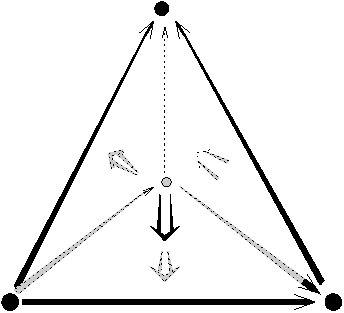
\includegraphics{figures/tetrahedron}
  \put(-127,46){${}_{g_{ij}}$}
  \put(-53,46){${}_{g_{jk}}$}
  \put(-90,-3){$g_{ik}$}
  \put(-137,80){$g_{il}$}
  \put(-41,80){$g_{kl}$}
  \put(-82,105){${}_{g_{jl}}$}

  \put(-80,22){$h_{ijk}$}
  \put(-82,47){$h_{ikl}$}
  \put(-68,85){${}_{h_{jkl}}$}
  \put(-112,85){${}_{h_{ijl}}$}
\end{picture}
\end{eqnarray*}

% \begin{displaymath}
%  \xymatrix@+4pc{
% & \bullet & \\
% & \ar@*{[|(20)]}[dr]^{g_{jk}} \ar[u]^{g_{jl}} & \\
% \ar[rr]_{g_{ik}} \ar[uur]^{g_{il}} \ar[ur]^{g_{ij}} & & \ar[uul]^{g_{kl}} \\}
% \end{displaymath}



\begin{definition}\label{g2bundle}
Let $\mathcal{G}$ be a smooth 2-group, and $\mathcal{F}$ a smooth space. A (strict) \define{action} of $\mathcal{G}$ in $\mathcal{F}$ is a smooth map \[
                        \alpha:\mathcal{G}\rightarrow \mathcal{AUT}(\mathcal{F})
                       \]
that preserves products and inverses (i.e., a \define{smooth homomorphism}).
We say that a locally trivial 2-bundle has \define{structure 2-group} $\mathcal{G}$, when $g,h$ and $k$ (defined above) factor through an action $\mathcal{G}\rightarrow\mathcal{AUT}(\mathcal{F})$. In this case, $E$ is said to be a \define{$\mathcal{G}$-2-bundle}. Furthermore, when $\mathcal{F}=\mathcal{G}$ it is said to be a  \define{principal $\mathcal{G}$-2-bundle}.
\end{definition}




\section{2-Bundles with 2-Connections}
%\improve{final version will change here, starting with diagrams which were temporarily borrowed}

In order to categorify the notion of holonomy we need the following description of a connection in terms of local holonomy functors from \cite{baez-2004}:

\begin{theorem}
Let $(E,p,B)$ be a principal $G$-bundle of smooth spaces with a smooth structure group, locally trivialized over a cover $\{ U_i\}_{i\in I}$ with corresponding transition functions $g_{ij}$. There is a bijection between connections on $E$ and smooth maps of 2-spaces \[
hol_i:P^1_1(U_i)\rightarrow G
\]
for each $i\in I$, such that:
each $g_{ij}$ defines a smooth natural isomorphism $hol_{i|U_{ij}}\rightarrow hol_{j|U_{ij}}$.
\end{theorem}

%% Recall that a connection assigned an element of the structure group to paths in the base space. We then expect a 2-connection to assign to each path an object of the structure 2-group, and to each ``surface'' a morphism. By ``surface'' we mean the following:

That is, the diagram below commutes, for every path $\gamma$ in $U_{ij}$ connecting $x$ and $y$.

\[
\xymatrix{\bullet \ar[rr]^{g_{ij}(x)} \ar[dd]_{hol_i(\gamma)} & & \bullet \ar[dd]^{hol_j(\gamma)}\\
\\
\bullet \ar[rr]_{g_{ij}(y)} & & \bullet
}
\]

And from the cocycle equation $g_{ik}=g_{ij}g_{jk}$,
\[
\xymatrix{ & hol_j \ar[ddr]^{g_{jk}} &\\
\\
hol_i \ar[uur]^{g_{ij}} \ar[rr]_{g_{ik}} & & hol_k}
\]

\begin{definition}
 Let $M$ be a smooth space. A \define{parametrized bigon} in $M$ is a smooth map\[
                                                                                 \Sigma:[0,1]\times [0,1]\rightarrow M
                                                                                \]
where $\Sigma(s,\cdotp)$ is constant for $s$ in a neighborhood of 0 and 1, and $\Sigma(s,t)$ is independent of $t$ when $t$ approaches 0 and 1. $\gamma_0=\Sigma(\cdotp,0)$ and $\gamma_1=\Sigma(\cdotp,1)$ are said to be the \define{source} and \define{target} of $\Sigma$ respectively. We write $\Sigma:\gamma_0\rightarrow \gamma_1$.
We generalize the notion of path groupoid again using the notion of thin homotopy.
\end{definition}
\begin{definition}
 Let $M$ be a smooth space, and $\Sigma:\gamma_0\rightarrow \gamma_1$ and $\Sigma':\gamma_0'\rightarrow \gamma_1'$ be parametrized bigons in $M$. A \define{thin homotopy} between $\Sigma$ and $\Sigma'$ is a smooth map $H:[0,1]^3\rightarrow M$ such that
\begin{itemize}
 \item $\text{rank}(dH(s,t,u))< 3$ for all $s,t,u$.
 \item $H(s,t,0)=\Sigma(s,t)$,
 \item $H(s,t,1)=\Sigma'(s,t)$,
\item $H(s,t,u)$ is independent of $u$ in a neighborhood of $u=0$ and 1, and it is constant near $s=0$ and 1,
\item for $t$ in a neighborhood of 0 we have that $H(s,t,u)=H_0(s,u)$ for some thin homotopy from $\gamma_0$ and $\gamma_0'$,
\item for $t$ in a neighborhood of 1 we have that $H(s,t,u)=H_1(s,u)$ for some thin homotopy from $\gamma_1$ and $\gamma_1'$,
\end{itemize}
As before this forms an equivalence relation, and two parametrized bigons $\Sigma,\Sigma'$ are said to have the same thin homotopy class if they are thinly homotopic. To a class of this relation we call a \define{bigon}, the class above being written $[\Sigma]$.
The \define{path 2-groupoid} $P_2(B)$ of a smooth space $B$ is the 2-category whose objects are the points of $B$, morphisms are thin homotopy classes of paths $[\gamma]$ in $B$ that are constant near the edges, and 2-morphisms are bigons in $B$, represented by (taking $x=\gamma(0)$, $y=\gamma(1)$)
\[
 \xymatrix{ x \ar@/^1pc/[rr]^{[\gamma_0]}_{}="0"
           \ar@/_1pc/[rr]_{[\gamma_1]}="1"
           \ar@{=>}"0";"1"^{[\Sigma]} && y}
\]
with the natural compositions (see \cite{baez-2004}).
\end{definition}

It is left to check that this has a structure of a smooth 2-category. Here we are implicitly stating the internalization process defined in the beginning has a straightforward generalization, so that a smooth 2-category is a 2-category internalized in $C^\infty$.

\begin{definition}
 Let $p:E\rightarrow B$ be a $\mathcal{G}$-2-bundle as in Definition \ref{g2bundle}, where for simplicity we assume that $k_i=1$. A \define{2-connection} is a tuple of the following:
%\improve{duvida}
\begin{itemize}
 \item Smooth 2-functors $hol_i:P_2(U_i)\rightarrow \mathcal{G}$,
\item Pseudonatural isomorphisms \[
                           g_{ij}:hol_i|_{P(U_{ij})}\rightarrow hol_j|_{P(U_{ij})}
                          \]
extending the transition functions. That is, for each $\gamma:x\rightarrow y$ in $U_{ij}$ a morphism

\begin{center}
\begin{picture}(100,100)
  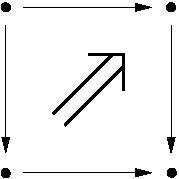
\includegraphics{figures/filled_square}
  \put(-60,90){$g_{ij}\of{x}$}
  \put(-60,-8){$g_{ij}\of{y}$}
  \put(-120,42){$\hol_i(\gamma)$}
  \put(0,42){$\hol_j(\gamma)$}
  \put(-75,50){$g_{ij}\of{\gamma}$}
\end{picture}
\vskip 0.5em
\end{center}
depending smoothly on the path $\gamma$, that makes the following diagram commute:\\
\begin{eqnarray*}
\begin{picture}(240,140)
 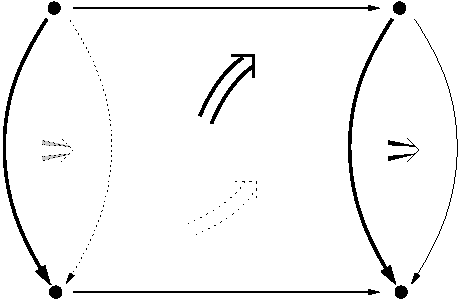
\includegraphics{figures/tincan}
 \put(-3,-17){	
 \begin{picture}(0,0)
 \put(122,0){
  \begin{picture}(0,0)
   \put(-385,90){$\hol_i\of{\gamma}$}
   \put(-290,100){${}_{\hol_i\of{\eta}}$}
   \put(-333,100){$\hol_i\of{\Sigma}$}
   \put(-242,50){${}_{g_{ij}\of{\eta}}$}
   \put(-268,125){${g_{ij}\of{\gamma}}$}
   \put(-250,163){$g_{ij}\of{x}$}
   \put(-250,10){$g_{ij}\of{y}$}
  \end{picture}}
 \put(288,0){
  \begin{picture}(0,0)
   \put(-382,90){$\hol_j\of{\gamma}$}
   \put(-290,100){${}_{\hol_j\of{\eta}}$}
   \put(-333,100){$\hol_j\of{\Sigma}$}
  \end{picture}}
 \end{picture}}
\end{picture}
\end{eqnarray*}
for any bigon $\Sigma: \gamma \Rightarrow \eta$ in $U_{ij}$,
\item modifications $h_{ijk}$ (induced by the transition functions $h_{ijk}$):
\[
 \xymatrix{& hol_j \ar[ddr]^{g_{jk}} \ar@{=>}[dd]^{h_{ijk}} &\\
\\
hol_i \ar[uur]^{g_{ij}} \ar[rr]_{g_{ik}} & & hol_k}
\]

That is, the following commutes:

\begin{center}
\begin{picture}(180,270)
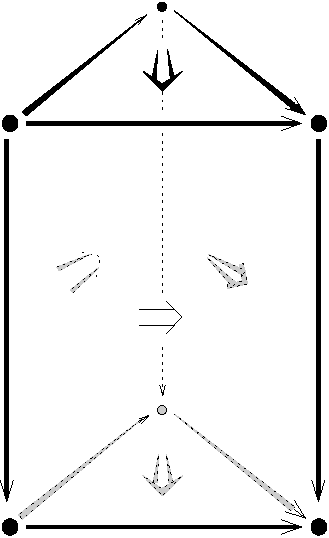
\includegraphics{figures/prism}
  \put(-3,100){$\hol_k\of{\gamma}$}
  \put(-190,100){$\hol_i\of{\gamma}$}
  \put(-80,160){${}_{\hol_j\of{\gamma}}$}
  \put(-100,-7){$g_{ik}\of{y}$}
  \put(-100,187){$g_{ik}\of{x}$}
  \put(-138,43){${}_{g_{ij}\of{y}}$}
  \put(-138,237){${}_{g_{ij}\of{x}}$}
  \put(-47,43){${}_{g_{jk}\of{y}}$}
  \put(-47,237){${}_{g_{jk}\of{x}}$}
  \put(-95,16){${}_{h_{ijk}\of{y}}$}
  \put(-95,212){${}_{h_{ijk}\of{x}}$}
  \put(-100,90){$g_{ik}\of{\gamma}$}
  \put(-150,124){${}_{g_{ij}\of{\gamma}}$}
  \put(-50,117){${}_{g_{jk}\of{\gamma}}$}
\end{picture}
\end{center}
for any bigon $\Sigma : \gamma \Rightarrow \eta$ in $U_{ijk}$.
\end{itemize}

\end{definition}

The following is one of the main results in \cite{baez-2004}.

\begin{theorem}
 Let $p:E\rightarrow B$ be a principal $\mathcal{G}$-2-bundle, locally trivial over an open cover $\{U_i\}$. Suppose that $k_i=1$. Let $(G,H,\partial,\vartriangleright)$ be the Lie crossed module associated to $\mathcal{G}$, with differential Lie crossed module $(\mathfrak{g},\mathfrak{h},\partial,\vartriangleright)$.

Then there is a one-to-one correspondence between 2-connections on $E$ and differential forms $(A_i,B_i,a_{ij})\in \Omega^1(U_i,\mathfrak{g})\times \Omega^2(U_i,\mathfrak{h})\times \Omega^1(U_{ij},\mathfrak{h})$ such that:
\begin{enumerate}
 \item \label{fakec} $F_{A_i}+\partial(B_i)=0$, where $F_{A_i}=dA_i+A_i\wedge A_i$ (the \define{curvature 2-form} of $A_i$).
\item $A_i=g_{ij}A_jg_{ij}^{-1}+g_{ij}dg_{ij}^{-1}-\partial (a_{ij})$
\item $B_i=g_{ij}\vartriangleright B_j+k_{ij}$ where $k_{ij}=da_{ij}+a_{ij}\wedge a_{ij}+d\alpha (A_i)\wedge a_{ij}$
\item $a_{ij}+g_{ij}\vartriangleright a_{jk}=h_{ijk}a_{ik}h_{ijk}^{-1}+(dh_{ijk})h_{ijk}^{-1}+(A_i\vartriangleright h_{ijk})h_{ijk}^{-1}$
\end{enumerate}
\end{theorem}

\future{\improve{ver relacao disto com o teorema do Picken para bundles com conexao. la o grupo de estrutura codificava o fibrado? e era a holonomia que dava a conexao. aqui fixamos o grupo...}}


\subsection{Gerbes}
%\improve{This section will be more developed in the final version}
\future{\improve{construcao toda no 2-bundles do bartels, pag. 74}}
This reduces to the case of \define{abelian gerbes}  with connections when $k_i=1$ and $F=\mathcal{G}$ is as in Example \ref{abgerb}. Similarly we arrive at \define{nonabelian gerbes} when $k_i=1$ and $F=\mathcal{G}$ is as in Example \ref{nabgerb}. Recall that equivalence classes of gerbes correspond bijectively to the elements in $\check{H}^2(M,\underline{S^1}_B)$ (see \cite[p. 10]{picken_parallel}).

\future{In \cite{bartels-2004} the 2-category of $\mathcal{G}$-2-bundles is defined and shown to be equivalent to the 2-category of abelian or nonabelian gerbes, when $\mathcal{G}$ is as above.
\improve{ver todas as condicoes. por exemplo, so englobam os gerbes com fake curvature (as introduced in \cite{breen-2001}), by condition (\ref{fakec})}.
 \improve{falar de fake curvature, de onde vem - Breen Messing}}

\newpage
\section{Categorical connections} \label{catconn}
We now focus on a particular kind of 2-connection introduced in \cite{picken_faria} by Martins and Picken, which can be used to define parallel transport. Here we address the question of the existence of such connections.

% Our construction corresponds to the particular case of $\mathcal{G}$-2-bundles introduced in \cite{picken_faria}, for which the $E$ valued transition functions are trivial, and therefore the $G-$valued transition functions satisfy the usual cocycle condition for a principal $G$-bundle. More specifically we will study a particular 2-connection in certain 2-bundles, as we hope to make clear later.

\begin{definition}
 Let $\mathcal{G}=(\partial :H\rightarrow G,\vartriangleright)$ be a crossed module, with associated differential crossed module $\mathfrak{G}=(\partial:\mathfrak{h}\rightarrow \mathfrak{g},\vartriangleright)$. A \define{$\mathcal{G}$-categorical connection} on a principal $G$-bundle $p:E \rightarrow B$ is a pair $(m,\omega)$ where $\omega\in \Omega^1(E,\mathfrak{g})$ is a connection 1-form on $E$ and $m$ is an equivariant horizontal 2-form in $\Omega^2(E,\mathfrak{h})$, such that
\begin{equation}
\partial (m)=\Omega \label{vanish}
\end{equation}
\end{definition}
By saying that $m$ is equivariant we mean that for all $g\in G$, $(R_g)^*m=g^{-1} \vartriangleright m$. It should be remarked that condition (\ref{vanish}) corresponds to the \emph{vanishing of the fake curvature} as introduced in \cite{breen-2001}.

\begin{definition}
 To a categorical connection as above, we associate the \define{2-curvature} 3-form as
\[
 \mathcal{M}=dm(H\times H\times H)
\]
\end{definition}


\begin{definition}\label{rw}
 Let $\omega \in \Omega^n(M,\mathfrak{g})$ and $\eta\in \Omega^m(M,\mathfrak{h})$. We define the \define{covariant tensor field} on $M$ with values in $\mathfrak{h}$ is defined by
\[
 (\omega\otimes^\vartriangleright \eta)(A_1,\ldots,A_n,B_1,\ldots,B_m)=\omega(A_1,\ldots,A_n)\vartriangleright \eta(B_1,\ldots,B_m), \quad A_i,B_i\in \mathfrak{X}(M)
\]
This gives us a natural \define{alternating tensor field} $\omega\wedge^\vartriangleright \eta \in \Omega^{n+m}(M,\mathfrak{h})$ with
\[
 \omega\wedge^\vartriangleright \eta=\frac{(n+m)!}{n!m!}\text{Alt}(\omega\otimes^\vartriangleright\eta)
\]
\end{definition}

\begin{example}
Let $\mathcal{G}=(\text{id}:G\rightarrow G,\vartriangleright)$, where $\vartriangleright$ is the adjoint action of $G$ on $G$.

Let $p:E\rightarrow B$ be principal $G$-bundle with connection one-form $\omega$. Then $(\omega,m)$ is a $\mathcal{G}$-categorical connection, where $m=\Omega$ is the curvature 2-form of $\omega$.

Note that in terms of Definition \ref{rw} the \define{structure equation} for the curvature form is
\[
 \Omega=d\omega +\frac{1}{2}\omega\wedge^{\text{ad}}\omega
\]
and the \define{Bianchi identity} is \[
                                          d\Omega+\omega\wedge^{\text{ad}}\Omega=0
                                         \]

\end{example}

\future{\improve{acima nao queria outro ``define'', mas um comando que voltasse a indexar o mesmo nome na mesma entrada}}

\begin{lemma}
 If $\varphi$ is a $G$-equivariant horizontal $(n-1)$-form in $P$, then
\[
 D\varphi =d\varphi +\omega \wedge^{\text{ad}}\varphi
\]

\end{lemma}


\begin{prop}[\index{2-structure equation}2-structure equation]
 \[\mathcal{M}=dm+\omega\wedge^{\vartriangleright}m \]
In particular $\mathcal{M}$ is $G$-equivariant.
\end{prop}

See \cite[p. 79]{kobayashi1} and \cite[p. 19]{picken_faria}.

% This follows partly from the following:
% 
% \begin{lemma}
%  If $\eta\in \Omega^{n-1}(E,\mathfrak{g})$ is $G$-equivariant, then $D\eta=d\eta+\omega\wedge^\vartriangleright \eta$.
% \end{lemma}
% 
% \improve{prove this later (?)}

\begin{prop}[\index{2-Bianchi identity}2-Bianchi identity]
 \[
  d\mathcal{M}(H\times H\times H\times H)=0
 \]
or by the previous lemma,
\[
 d\mathcal{M}+\omega\wedge^\vartriangleright \mathcal{M}=0.
\]
\end{prop}

\subsection{Local forms of the categorical connection}
Take an open cover $\{U_\alpha\}_\alpha$ of $B$ that trivializes our bundle. Taking local sections $f_\alpha:U_\alpha\rightarrow E_\alpha$, the local forms are given by \[
              m_\alpha=(f_\alpha)^*m
		   \]
\[
 \omega_\alpha=(f_\alpha)^*\omega
\]

We have already characterized the local form of $\omega$ and $\Omega$. Note that, defining  $\phi_{\alpha,\beta}:U_{\alpha,\beta}\rightarrow G$ by $f_\alpha (x)\phi_{\alpha,\beta}(x)=f_\beta(x)$,  from the $G$-invariance of $m$ and $\mathcal{M}$ we get:

\[
 m_\beta(X,Y)=\phi_{\alpha,\beta}^{-1}\vartriangleright m_\alpha(X,Y)
\]
\[
 \mathcal{M}_\beta (X,Y,Z)=\phi_{\alpha,\beta}^{-1}\vartriangleright \mathcal{M}_\alpha(X,Y,Z)
\]
for each $X,Y\in \mathfrak{X}(U_{\alpha\beta})$.


\begin{prop}\label{localform}
 Let $H,G$ be Lie groups, $B$ a smooth manifold and $E\rightarrow B$ a principal $G$-bundle. Let $\mathscr{G}=(\partial:H\rightarrow G,\vartriangleright)$ be a Lie crossed module and $\mathfrak{G}=(\partial:\mathfrak{h}\rightarrow\mathfrak{g},\triangleright)$ its associated differential crossed module.
Then a pair $(\omega,m)\in \Omega^2(E,\mathfrak{g})\times \Omega^1(E,\mathfrak{h})$ is a $\mathscr{G}-$categorical connection on $E$ if and only if there are local sections $f_\alpha:U_\alpha\rightarrow E_\alpha$ of $E$ (where $\{U_\alpha\}_\alpha$ is an open cover of $B$) and local forms $(\omega_\alpha,m_\alpha)\in \Omega^1(U_\alpha,\mathfrak{g})\times\Omega^2(U_\alpha,\mathfrak{h})$ with the following properties for each $U_{\alpha\beta}\neq\emptyset$: defining $\phi_{\alpha,\beta}:U_{\alpha,\beta}\rightarrow G$ by $f_\alpha (x)\phi_{\alpha,\beta}(x)=f_\beta(x)$, 

\begin{align}
 \partial(m_\alpha)&=\Omega_\alpha=d\omega_\alpha+\frac{1}{2}\omega_\alpha\wedge^{ad} \omega_\alpha \label{partialomega} \\
 \omega_\beta(X)&=\phi^{-1}_{\alpha,\beta}\omega_\alpha(X)\phi_{\alpha,\beta}+\phi^{-1}_{\alpha,\beta}d\phi_{\alpha,\beta} \label{connection}\\
 m_\beta(X,Y)&=\phi^{-1}_{\alpha,\beta}\triangleright m_\alpha(X,Y) \label{compatform}
\end{align}
for each $X,Y\in \mathfrak{X}(B)$.
\end{prop}
\begin{lemma}
Let $(E,p,B)$ be the trivial bundle $E=B\times G$. Given $(\omega_0,m_0)\in \Omega^1(B,\mathfrak{g})\times \Omega^2(B,\mathfrak{h})$ such that $\partial(m_0)=\Omega_0$, there exists a $\mathcal{G}$-categorical form $(\omega,m)$ with local forms $(\omega_0,m_0)$.
\end{lemma}
\begin{proof}

Let $\theta$ be the canonical left invariant $\mathfrak{g}$-valued form on $G$ (see Equation (\ref{maurercartan})). Let $f:B\rightarrow E$ be the trivial section $f(x)=(x,e)$ (where $e$ is the identity of $G$). Then $\omega_{(x,g)}=g^{-1}p^*(\omega_0)g+\theta$ is a connection 1-form on $E=M\times G$ with local form $\omega_0$ (this is a classical construction, see \cite[p. 67]{kobayashi1}).
Define $m$ for any $(x,g)\in B\times G$ and $X,Y\in T_{(x,g)}E$ by \[
m(X,Y)=g^{-1}\vartriangleright p^*(m_0)(X,Y)
\]
This 2-form is horizontal since clearly $p^*(m_0)$ is horizontal. For $G$-invariance, let $X,Y\in T_{(x,g)}E$.
\begin{align*}
 (R_h^*m)_g(X,Y)&=m_{gh}(Xh,Yh)\\
&=(gh)^{-1}\vartriangleright p^*(m_0)(Xh,Yh)\\
&=h^{-1}g^{-1}\vartriangleright p^*(m_0)(X,Y)\\
&=h^{-1}\vartriangleright m(X,Y)
\end{align*}

Also recall that $\Omega(X,Y)=g^{-1}p^*(\Omega_0)(X,Y)g$, therefore:
\begin{align*}
\partial (m) (X,Y)&= \partial(g^{-1}\vartriangleright p^*(m_0)(X,Y))\\
& =g^{-1}\partial (p^*(m_0)(X,Y)) g\\
& =g^{-1}p^*(\partial(m_0))(X,Y) g\\
& =g^{-1}p^*(\Omega_0)(X,Y)g\\
& =\Omega(X,Y)
\end{align*}

\end{proof}

%  \notsute{is an cover  $\{U_\alpha\}$ of $M$ such that $E_\alpha=E|U_\alpha$ is trivial}, and local sections $f_\alpha:U_\alpha\rightarrow E_\alpha$ of $P$ (defining $\phi_{\alpha,\beta}:U_{\alpha,\beta}\rightarrow G$ by $f_\alpha (x)\phi_{\alpha,\beta}(x)=f_\beta(x)$
% 
% $(\omega_\alpha,m_\alpha)\in \Omega^1(U_\alpha,\mathfrak{g})\times\Omega^2(U_\alpha,\mathfrak{e})$ 
% 	
%  such that for $U_{\alpha,\beta}\neq\emptyset$:
% \begin{align*}
%  \partial(m_\alpha)&=\Omega_\alpha=d\omega_\alpha+\frac{1}{2}\omega_\alpha\wedge^{ad} \omega_\alpha \\
%  \omega_\beta(X)&=\phi^{-1}_{\alpha,\beta}\omega_\alpha(X)\phi_{\alpha,\beta}+\phi^{-1}_{\alpha,\beta}d\phi_{\alpha,\beta}\\
%  m_\beta(X,Y)&=\phi^{-1}_{\alpha,\beta}\triangleright m_\alpha(X,Y)
% \end{align*}


\subsection{Existence}\label{existence}
A connection 1-form on any bundle can always be found by the means of partitions of unity (see for instance \cite[p. 67]{kobayashi1}). Our problem lies with the form $m$. For that, we describe it in the following terms (as in \cite[p. 75]{kobayashi1}).

\begin{definition}\label{tensdef}
Let $(E,p,B)$ be a principal $G$-bundle. Let $(\rho,V)$ be a representation of $G$ in a finite dimensional vector space $V$. A \define{tensorial form} of degree $k$ on $E$ of type $(\rho,V)$ is a form $\varphi\in\Omega^k (E,V)$ such that
\begin{itemize}
\item $\varphi$ is $G$-invariant for the induced action of $G$ on $V$, i.e. $R_g^*=\rho(g^{-1})\varphi$,
\item $\varphi$ is horizontal, i.e. $\varphi(X_1,\ldots,X_k)=0$ when one of the tangent vectors $X_i$ is vertical.
\end{itemize}
\end{definition}

\begin{example}\label{tensorialexample}
A connection $\omega$ is a tensorial form of degree 1 in $E$ of type $(\text{Ad},\mathfrak{g})$. By definition, $m$ is a tensorial form of degree 2 in $E$ of type $(\vartriangleright,\mathfrak{h})$.
\end{example}


\begin{lemma}\label{tensorialform}
Let $(E',q,B)$ be the bundle associated with the principal $G$-bundle $(E,p,B)$ with fibre $V$, where $G$ acts naturally by $\rho$. There is a one-to-one correspondence between the tensorial forms as above and sections of the bundle \[
\xymatrix{\wedge^k T^*B\otimes E' \ar[d]\\
B} \]
\end{lemma}

\begin{proof}
The associated bundle with fibre $V$ has total space $E'=E \times V / \sim$ where $(eg,x)\sim (e,gx)$. Then each $u\in E$ defines a linear mapping $V\rightarrow q^{-1}(x)$, where $x=p(u)$ given by $ v\mapsto [(u,v)] $


A tensorial $(\rho,V)$ form of degree $k$ can be regarded as a skew-symmetric multilinear mapping $\widetilde{\varphi}_x: T_x(B)\times \ldots \times T_x(B) \rightarrow q^{-1}(x)$, putting
\[
\widetilde{\varphi}_x(X_1,\ldots,X_k)=u(\varphi(X_1^*,\ldots, X_k^*)), \qquad X_i \in T_x(B)
\]letting $X_i^*$ be any vectors at $u$ such that $p(X_i^*)=X_i$. One verifies that this does not depend on the choice of $u$ or the $X_i^*$'s. Conversely, given $\widetilde{\varphi}_x:T_x(B)\times\ldots\times T_x(B)\rightarrow q^{-1}(x)$ skew-symmetric and multilinear, one obtains a tensorial form of degree $k$ of type $(\rho,V)$ on $E$ defined by
\[
\varphi(X_1^*,\ldots,X_k^*)=u^{-1}(\widetilde{\varphi}_x(p(X_1^*),\ldots,p(X_k^*))), \qquad X_i^*\in T_uE
\]
\end{proof}
\future{\improve{acima escolher melhor a construcao}}


Let \index{$\mathfrak{b}$} $\mathfrak{b}=\text{Ker }\partial$ and fix a connection $\omega$. One immediately notices that for any 2-forms $m, m'\in \Omega^2(E,\mathfrak{h})$ of categorical connections with connection $\omega$, $m-m'$ is in $\Omega^2(E,\mathfrak{b})$. Moreover, given such a 2-form $m$, all others are in $\{m+m_0: m_0\in \Omega^2(E,\mathfrak{b})\}$.
\begin{corollary}
For a connection $\omega$, if the set of forms $m$, such that $(\omega,m)$ is a categorical connection, is non-empty, then it is an affine space over $\Gamma_B(\wedge^2T^*B\otimes \mathfrak{b})$.
\end{corollary}

%% \begin{prop}
%% Let $\xi=(E,p,B)$ be a \notsure{fibre bundle} with connection $\omega$, and let $\mathcal{G}=(\partial:E\rightarrow G)$ a Lie crossed module. The following are equivalent:
%% \begin{enumerate}
%% \item There is a $\mathcal{G}$-categorical connection on $\xi$ with connection $\omega$. \label{1}
%% \item $\text{Im}(\Omega)\subset \mathfrak{a}$, where $\mathfrak{a}=\text{Im }\partial$ \index{$\mathfrak{a}$} \notsure{CHECK, only these??}.\label{2}
%% \item $\xi$ admits a reduction to a structure group $H\subset G$, with Lie algebra $\mathfrak{h}$ contained in $\mathfrak{a}$. \label{3}
%% \end{enumerate}
%% \end{prop}
%% \begin{proof}
%% "Connections always exist".... comment, say below .
%% $(\ref{1})\Rightarrow (\ref{2})$ follows by definition. Suppose $\text{Im}(\Omega)\subset \mathfrak{a}$. By Lemma (\ref{tensorialform})b
%% \end{proof}

\begin{theorem}\label{mainthm}
Let $\xi=(E,p,B)$ be a principal $G$-bundle, and let $\mathcal{G}=(\partial:H\rightarrow G)$ a Lie crossed module. The following are equivalent:
\begin{enumerate}
\item There is a $\mathcal{G}$-categorical connection on $\xi$. \label{1}
\item $\xi$ admits a connection with curvature $2$-form $\Omega$ such that $\text{Im}(\Omega)\subset \mathfrak{a}$, where $\mathfrak{a}=\text{Im }\partial$ \index{$\mathfrak{a}$}.\label{2}
\item $\xi$ admits a reduction to a structure group $G'\subset G$, with Lie algebra $\mathfrak{g}'$ contained in $\mathfrak{a}$. \label{3}
\end{enumerate}
\end{theorem}
\begin{proof}\hspace*{\fill}\\ \begin{itemize}
\item[\footnotesize{$(\ref{1})\Rightarrow (\ref{2})$}] Follows by definition. 
\item[\footnotesize{$(\ref{2})\Rightarrow (\ref{1})$}] Let $(E_1,p_1,B)$ be the associated bundle with fibre $\mathfrak{e}$, and $(E_2,p_2,B)$ with fibre $\mathfrak{a}$. Recall that $E_1=E\times_G \mathfrak{h}$ and $E_2=E\times_G \mathfrak{a}$. $m$ corresponds to a 2-form with values in $E_1$, while $\Omega$ corresponds to a 2-form with values in $E_2$. Since $\partial$ is equivariant, the obvious surjective morphism $\widetilde{\partial}:E_1\rightarrow E_2$ is well defined. 
Now the problem of finding $m$ corresponds to the problem of finding a 2-form with values in $E_1$ that projects to the 2-form corresponding to $\Omega$. But applying Theorem \ref{exactseq} with $\xi=Ker \widetilde{\partial}, \chi=E_1$ and $\eta=E_2$ the projection has a right section $w$, and therefore we can take $m=\omega\circ\Omega$.
\item[\footnotesize{$(\ref{2})\Rightarrow (\ref{3})$}] Let $Hol$ be the holonomy group. By the reduction theorem \ref{redthm}, there is a reduction of the structure group to $Hol$. If $\mathfrak{h}$ denotes its Lie algebra, by Ambrose-Singer (Theorem \ref{ambrosesinger}) and since $\Omega$ is horizontal $\mathfrak{h}=\text{Im } \Omega \subset \mathfrak{a}$.
\item[\footnotesize{$(\ref{3})\Rightarrow (\ref{1})$}] If there is a reduction of the structure group $G$ to $G'$, let $\{U_{\alpha\beta}\}$ be a cover with transition functions $g_{\alpha\beta}$ of $\xi$ with values in $G'$ (which exists by Proposition \ref{redprop}). Denoting the Lie algebra of $Hol$ of the reduced bundle by $\mathfrak{h'}$, we get again by Ambrose-Singer that \[
Im \Omega=\mathfrak{h}'\subset \mathfrak{g}' \subset \mathfrak{a}
\] Then the reduced bundle has a categorical connection (by the equivalence of (1) and (2) proved earlier), and by Proposition \ref{localform} we see that the local categorical connection forms of the cover $\{U_{\alpha\beta}\}$, are also local categorical connection forms on $\xi$.
             \end{itemize}
\end{proof}
It should be noted that the above proof (together with the results used) is constructive.


Alternatively we could have proved $(\ref{3})\Rightarrow (\ref{2})$ by using the fact that the connection in the reduced bundle induces naturally a connection on the bundle by $G$-invariance (it is defined solely by its value in a point in each fibre) together with the main property of the fundamental vector field (see equation \ref{mainproperty}).

\begin{corollary}
 In the conditions of Theorem \ref{mainthm}, if $\partial:\mathfrak{e}\rightarrow \mathfrak{g}$ is surjective there is always a categorical connection on a bundle with structure group $G$.
\end{corollary}

This is the case of the crossed modules in Examples \ref{abgerb} and \ref{trivcross}. Most importantly, a categorical connection doesn't always exist.
\begin{example}
 Let $(H,.)=(\mathbb{R}^n,+)$ and $(G,.)=(GL(n,\mathbb{R}),\circ)$. Take the trivial map $\partial:H\rightarrow G$ together with the action $f\vartriangleright e=f(e)$ of $GL(n,\mathbb{R})$ in $\mathbb{R}^n$. Clearly $\mathcal{G}=(\partial:H\rightarrow G,\vartriangleright)$ is a crossed module. Since $\partial:\mathfrak{h}\rightarrow \mathfrak{g}$ is the zero map, in order for there to be a categorical connection, the holonomy group would have to be a discrete subgroup of $G$. But in general that is not the case: take for instance the frame bundle over $S^2$, with $G=GL(2,\mathbf{R})$ and $H=(\mathbf{R}^2,+)$. If the frame bundle could be reduced to a discrete group then it would be trivial as, for any topological group, principal $G$-bundles over $S^2$ are classified by conjugacy classes in $\pi_1(G)$. In particular there would be a section of the frame bundle and hence a nowhere vanishing tangent vector field to $S^2$ which is impossible by the hairy ball theorem (see Theorem (2.28) in \cite[p. 135]{hatcher}).
\end{example}


\subsubsection{Construction for compact groups}

%% We now try to obtain $\mathscr{G}$-categorical connections on a principal $G$-bundle $E\rightarrow M$, with $E,G$ Lie groups. Notice that a connection one-form $\omega$ of the bundle can always be found with the use of partition functions. Also a choice of local forms $\omega_\alpha\in \Omega(U_\alpha,\mathfrak{g})$ such that (\ref{connection}) is equivalent to a choice of a one-form connection on the bundle. So the problem of finding a $\mathscr{G}$-categorical connection reduces to the problem of finding the 2-form $m$. Let $A=\partial(E)$ and $B=Ker(\partial)\subset E$, with corresponding Lie algebras $\mathfrak{a},\mathfrak{g}$. It is a necessary condition for the existence of a categorical connection that $Im(\Omega)\subset \mathfrak{a}$, so let us assume it is the case. 
In the case where categorical connections exist, we provide an alternative way of getting one when the structure group $G$ is compact.
Notice that a local form $m_\alpha\in \Omega^2(U_\alpha,\mathfrak{e})$ satisfies (\ref{partialomega}) if and only if it is of the form
\[ m_\alpha=r\Omega_\alpha+\varphi_\alpha \]
for a left section $r:\mathfrak{a}\rightarrow \mathfrak{e}$ of $\partial$ (ie, $\partial r=id_\mathfrak{a}$) and a local form $\varphi_\alpha\in\Omega^2(U_\alpha,\mathfrak{b})$.
% for any local trivializations $f_\alpha:U_\alpha\rightarrow E_\alpha$, putting $\omega_\alpha=f^*_\alpha \omega \in \Omega(U_\alpha,\mathfrak{g})$ condition \ref{connection} is automatically satisfied, in fact 
% 
% \improve{ter o $\omega$ e o mesmo que ter os $\omega_\alpha$ com (\ref{connection}) certo?}
We can write (\ref{compatform}) in the form:

\[
 (r\Omega_\beta (X,Y)+\varphi_\beta(X,Y))=\phi_{\alpha,\beta}^{-1}\vartriangleright(r\Omega_\alpha (X,Y))+\phi_{\alpha,\beta}^{-1}\vartriangleright \varphi_\alpha(X,Y)
\]

So it would be sufficient to get
\begin{align}
          r\Omega_\beta(X,Y)&=\phi_{\alpha,\beta}^{-1}\vartriangleright (r\Omega_\alpha)(X,Y) \label{eq} \\
        \varphi_\beta (X,Y)&=\phi_{\alpha,\beta}^{-1}\vartriangleright \varphi_\alpha (X,Y) 
\end{align}

But $\Omega_\beta(X,Y)=\phi_{\alpha,\beta}^{-1}\Omega_\alpha (X,Y)\phi_{\alpha,\beta}=Ad_{\phi_{\alpha,\beta}} \Omega_\alpha(X,Y)$
% for the adjoint action $\circ$:\begin{align*}
%                 G\times \mathfrak{g}&\rightarrow \mathfrak{g}\\
%                (g,v)&\mapsto Ad_g(v)
%                \end{align*}
where $Ad_g$ is the adjoint representation of $G$, the canonical action of $G$ in $\mathfrak{g}$.
\future{\improve{dizer o que e uma representacao}}
% , or the derivative in $e\in G$ of the action $g\in G\mapsto(v\mapsto g^{-1}hg))$.
%with an open cover $\{U_\alpha\}$ such that $P|U_\alpha$ is trivial

So condition (\ref{eq}) is verified when $r$ is $G$-equivariant.

\begin{lemma}
Let $G$ be a compact Lie group acting on $V,W$ linear spaces. Let $T:V\rightarrow W$ be an equivariant linear map. Then there is an equivariant left inverse $R:Im(T)\rightarrow V$ of $T$.
\end{lemma}
\begin{proof}
 Put $A=Im(T)$. One can always find a linear section $R_0$, not necessarily equivariant. In general an equivariant map $f:A\rightarrow V$ is a fixed point of the action $\circ$ given by
\begin{align*}
 G\times Hom(A,V)&\rightarrow Hom(A,V)\\
(g,f)&\mapsto (g\circ f)=(v\mapsto g.f(g^{-1}.v))
\end{align*}
Let $\int (\cdotp) dG$ be the unique (normalized) left-invariant integral on $G$ (see \cite[p. 41]{brocker}).
Define
\begin{align*}
 R:A&\rightarrow V\\
a&\mapsto \int_G\frac{g R_0(g^{-1}a)}{Vol(G)}dg
\end{align*}
It is clearly linear, and by left-invariance of the integral:
\begin{align*}
 (h\circ R)(a)&= hR(h^{-1}a)\\
              &= \int_G \frac{hg R_0((hg)^{-1}a)}{Vol(G)}dg\\
              &= \int_G \frac{g R_0(g^{-1}a)}{Vol(G)}dg\\
	      &= R(a)
\end{align*}

It is also a left inverse since, fixing a base of $V$, $T$ is represented by a matrix $(T_{ij})_{ij}$ and
\begin{align*}
 (T R)(a)&=T\int_G \frac{g R_0(g^{-1}a)}{Vol(G)}dg\\
         &=(T_{ij})_{ij}(\int_G \frac{R_0(g^{-1}a)}{Vol(G)} dg)_{i}\\
         &=(\sum_j T_{ij} \int_G (\frac{R_0(g^{-1}a)}{Vol(G)})_i dg)_i\\
         &=\int_G T(\frac{g R_0(g^{-1}a)}{Vol(G)})dg\\
         &=\int_G \frac{gTR_0(g^{-1}a)}{Vol(G)}dg \\
         &=\int_G \frac{gg^{-1}a}{Vol(G)}dg\\
         &= a
\end{align*}
\end{proof}
With the section given by this proposition, and taking all $\varphi_\alpha$ to be null, we get a connection 2-form $m$ compatible with a given $\omega$ .

\subsubsection{General local construction} Given a categorical connection we will locally construct other categorical connections with the same curvature.  We observed that any two $\mathscr{G}$-categorical connections $(\omega,m)$ and $(\omega,m')$ differ only on an horizontal and equivariant 2-form $\psi=m-m'\in\Omega^2(E,\mathfrak{b})$. There is a correspondence between these forms and the local forms $\psi_\alpha=m_\alpha-m_\alpha'$ (given by $\psi_\alpha=s_\alpha^*\psi$) obeying
\begin{equation}\label{psi}
\psi_\beta=\phi_{\alpha,\beta}^{-1}\vartriangleright \psi_\alpha                                                                                                                                                                                                                                                                                                                                                                                                                                                                                                                                                                               \end{equation}
That is, for a fixed local form  $(\omega_\alpha,m_\alpha)$ of $\mathscr{G}$-categorical connections, any other over the same $\omega$ will be of the form $(\omega_\alpha,m_\alpha+\psi_\alpha)$ for $\psi_\alpha\in\Omega^2(U_\alpha,\mathfrak{b})$ obeying (\ref{psi}).

Since $M$ is second countable it has countable open covers $\{U_i\}_i$ and $\{V_i\}_i$ such that $\bar{V}_i\subset U_i$. Let $m_{i}=s_i^*m$. Then at $U_0$, start with the 2-form $m'_0\in\Omega^2(U_0,\mathfrak{b})$ 
\[
 m_0'=m_{0}+\psi_0
\]
for \emph{any} $\psi_0\in\Omega^2(U_0,\mathfrak{b})$, where $m_0$ is the local form of our initial categorical connection. 

Next for $m'_1=m_1+\psi_1$, our choice of $\psi_1$ has to be an extension of $\phi_{01}^{-1}\vartriangleright\psi_0$. 



Let $\{v_i\}_j$ be a basis for $\mathfrak{b}$, so that $\psi_1=\sum_j \theta_j v_j$ for some 2-forms $\theta_j\in\Omega^2(U_1,\mathbb{R})$. Using local coordinates $x_1,\ldots,x_n$ in $U_1$, this becomes $\sum_j f_jdx_j$ for some smooth functions $f_j:U_{01}\rightarrow \mathbb{R}$. Considering instead the closed subset $\bar{V}_0\cap U_1$ in $U_1$, this reduces the problem to the following lemma, found on Appendix 3 of \cite{kobayashi1}:
\begin{lemma}\label{closed}
 Every differentiable function defined on a closed subset of $\mathbb{R}^n$ can be extended to a differentiable function on $\mathbb{R}^n$.
\end{lemma}

Assume having found $\{\psi_j\}_{j\leq i}$, with $\psi_j\in\Omega^2(U_j,\mathfrak{b})$ related by $\psi_k=\phi_{jk}^{-1}\vartriangleright \psi_j$ in $V_{jk}\neq\emptyset$.
Then we need to extend $\psi_{i+1}'=\phi_{j(i+1)}^{-1}\vartriangleright\psi_{j}$ from $U_{i+1}\cap \bar{V}_{0}\cup\ldots\cup \bar{V}_i$ to $U_{i+1}$. Note that this extension does not depend on $j\leq i$ since:\begin{align*}
\phi_{j(i+1)}^{-1}\vartriangleright\psi_j =(\phi_{jj'}\phi_{j'(i+1)})^{-1}\vartriangleright \psi_j=\phi_{j'(i+1)}^{-1}\vartriangleright (\phi_{jj'}^{-1}\vartriangleright\psi_j)=\phi_{j'(i+1)}^{-1}\vartriangleright\psi_{j'}
\end{align*}
Then we proceed as before and apply the previous lemma. We have defined inductively a local form of a $\mathscr{G}$-categorical connection on the cover $\{V_i\}_i$.


\subsection{Relation with 2-bundles}
In \cite{picken_faria} the main goal was to construct a smooth map $P_2(B)\rightarrow \mathcal{G}$, where $P_2(B)$ is the path 2-groupoid of $B$, that unlike Baez's holonomy is defined in all of $B$. But this requires the existence of a smooth group morphism $\pi_1^1(B)\rightarrow G$, which by Theorem \ref{bundle121} requires the existence of a principal $G$-bundle with connection.
Using the passage from 2-groups to crossed modules (see Section (\label{passage})), a $\mathcal{G}$-2-bundle for a Lie crossed module $\mathcal{G}=(\partial:E\rightarrow G,\vartriangleright)$ is described by smooth maps $g_{ij}:U_{ij}\rightarrow G$ and $\tilde{h}_{ijk}:U_{ijk}\rightarrow E$ satisfying $\partial(h_{ijk})g_{ij}g_{jk}=g_{ik}$ and, by Equation (\ref{cococycle}),

\begin{align*}
  ((g_{ij}g_{jk},\tilde{h}_{ijk})\circ(g_{kl},1))\bullet(g_{ik}g_{kl},\tilde{h}_{ikl}) &=((g_{ij},1)\circ(g_{jk}g_{kl},\tilde{h}_{jkl}))\bullet(g_{ij}g_{jl},\tilde{h}_{ijl}) & \Leftrightarrow \\
 (g_{ij}g_{jk}g_{kl},\tilde{h}_{ijk})\bullet(g_{ik}g_{kl},\tilde{h}_{ikl}) &= (g_{ij}g_{jk}g_{kl},g_{ij}\vartriangleright \tilde{h}_{jkl})\bullet(g_{ij}g_{jl},\tilde{h}_{ijl}) & \Leftrightarrow\\
 (g_{ij}g_{jk}g_{kl},\tilde{h}_{ikl}\tilde{h}_{ijk})& =(g_{ij}g_{jk}g_{kl},\tilde{h}_{ijl}(g_{ij}\vartriangleright \tilde{h}_{jkl})) &\Leftrightarrow \\
\tilde{h}_{ijk}\tilde{h}_{ikl} &=(g_{ij}\vartriangleright \tilde{h}_{jkl})\tilde{h}_{ijl},  
\end{align*}

where $\bullet$ and $\circ$ are the associated vertical and horizontal compositions respectively.

Then we get a bundle if and only if $\partial(h_{ijk})=1$. 2-bundles of this type are called \define{special $\mathcal{G}$-2-bundles}. Thus categorical connections are a particular kind of 2-connection on a subclass of 2-bundles, namely special 2-bundles.
% Weakening our definition of $m$ to local forms $m_i\in\Omega^2(E_i,\mathfrak{h})$ still with $\partial(m_i)=\Omega_i$, then one passes to the 2-bundles context in the natural way (see \cite[p. 37]{picken_faria}).

%\improve{tirar citacoes a mais}

\addcontentsline{toc}{chapter}{Bibliography}
\nocite{*}
\bibliographystyle{alpha}
\bibliography{bibliography}  

\printindex
	
 
\end{document}
